% !TeX encoding = UTF-8
% !TeX program = latexmk
% !TeX spellcheck = en_US

\documentclass[degree=bachelor]{thuthesis}
  % 学位 degree:
  %   doctor | master | bachelor | postdoc
  % 学位类型 degree-type:
  %   academic(默认)| professional


% 论文基本配置,加载宏包等全局配置
% !TeX root = ../main.tex

% 论文基本信息配置

\thusetup{
  %******************************
  % 注意:
  %   1. 配置里面不要出现空行
  %   2. 不需要的配置信息可以删除
  %******************************
  %
  % 标题
  %   可使用“\\”命令手动控制换行
  %
  title  = {云网络下的异常检测系统设计与实现},
  title* = {Design and Implementation of Anomaly Detection System under Cloud Networks},
  %
  % 学位
  %   1. 学术型
  %      - 中文
  %        需注明所属的学科门类,例如:
  %        哲学、经济学、法学、教育学、文学、历史学、理学、工学、农学、医学、
  %        军事学、管理学、艺术学
  %      - 英文
  %        博士:Doctor of Philosophy
  %        硕士:
  %          哲学、文学、历史学、法学、教育学、艺术学门类,公共管理学科
  %          填写“Master of Arts“,其它填写“Master of Science”
  %   2. 专业型
  %      直接填写专业学位的名称,例如:
  %      教育博士、工程硕士等
  %      Doctor of Education, Master of Engineering
  %   3. 本科生不需要填写
  %
  % degree-name  = {工学硕士},
  % degree-name* = {Master of Science},
  %
  % 培养单位
  %   填写所属院系的全名
  %
  department = {计算机科学与技术系},
  %
  % 学科
  %   1. 学术型学位
  %      获得一级学科授权的学科填写一级学科名称,其他填写二级学科名称
  %   2. 工程硕士
  %      工程领域名称
  %   3. 其他专业型学位
  %      不填写此项
  %   4. 本科生不需要填写
  %
  discipline  = {计算机科学与技术},
  discipline* = {Computer Science and Technology},
  %
  % 姓名
  %
  author  = {赵\hbox{\lower-0.67ex\hbox{\scalebox{1}[0.6]{均}}\lower.2ex\hbox{\kern-1em \scalebox{1}[0.5]{金}}}峰},
  author* = {Zhao Yunfeng},
  %
  % 指导教师
  %   中文姓名和职称之间以英文逗号“,”分开,下同
  %
  supervisor  = {王之梁\ 副教授},
  %
  % 副指导教师
  %
  % associate-supervisor  = {陈文光教授},
  % associate-supervisor* = {Professor Chen Wenguang},
  %
  % 联合指导教师
  %
  % joint-supervisor  = {某某某教授},
  % joint-supervisor* = {Professor Mou Moumou},
  %
  % 日期
  %   使用 ISO 格式;默认为当前时间
  %
  % date = {2019-07-07},
  %
  % 密级和年限
  %   秘密, 机密, 绝密
  %
  % secret-level = {秘密},
  % secret-year  = {10},
  %
  % 博士后专有部分
  %
  % clc                = {分类号},
  % udc                = {UDC},
  % id                 = {编号},
  % discipline-level-1 = {计算机科学与技术},  % 流动站(一级学科)名称
  % discipline-level-2 = {系统结构},          % 专业(二级学科)名称
  % start-date         = {2011-07-01},        % 研究工作起始时间
}

%% Put any packages you would like to use here

% 表格中支持跨行
\usepackage{multirow}

% 跨页表格
\usepackage{longtable}

% 固定宽度的表格
\usepackage{tabularx}

% 表格中的反斜线
\usepackage{diagbox}

% 确定浮动对象的位置,可以使用 H,强制将浮动对象放到这里(可能效果很差)
\usepackage{float}

% 浮动图形控制宏包。
% 允许上一个 section 的浮动图形出现在下一个 section 的开始部分
% 该宏包提供处理浮动对象的 \FloatBarrier 命令,使所有未处
% 理的浮动图形立即被处理。这三个宏包仅供参考,未必使用:
% \usepackage[below]{placeins}
% \usepackage{floatflt} % 图文混排用宏包
% \usepackage{rotating} % 图形和表格的控制旋转

% 定理类环境宏包
\usepackage[amsmath,thmmarks,hyperref]{ntheorem}

% 支持算法
\usepackage{algorithm}
\usepackage{algorithmicx}
\usepackage{algpseudocode}
\usepackage{fixltx2e}
\usepackage{pdfpages}
%\usepackage{mathabx}

\renewcommand{\algorithmicrequire}{\textbf{输入:}}
\renewcommand{\algorithmicensure}{\textbf{输出:}}
\MakeRobust{\Call}

\makeatletter
\def\widebreve{\mathpalette\wide@breve}
\def\wide@breve#1#2{\sbox\z@{$#1#2$}%
     \mathop{\vbox{\m@th\ialign{##\crcr
\kern0.08em\brevefill#1{0.8\wd\z@}\crcr\noalign{\nointerlineskip}%
                    $\hss#1#2\hss$\crcr}}}\limits}
\def\brevefill#1#2{$\m@th\sbox\tw@{$#1($}%
  \hss\resizebox{#2}{\wd\tw@}{\rotatebox[origin=c]{90}{\upshape(}}\hss$}

\newenvironment{breakablealgorithm}
  {% \begin{breakablealgorithm}
   \begin{center}
     \refstepcounter{algorithm}% New algorithm
     \hrule height.8pt depth0pt \kern2pt% \@fs@pre for \@fs@ruled
     \renewcommand{\caption}[2][\relax]{% Make a new \caption
       {\raggedright\textbf{\ALG@name~\thealgorithm} ##2\par}%
       \ifx\relax##1\relax % #1 is \relax
         \addcontentsline{loa}{algorithm}{\protect\numberline{\thealgorithm}##2}%
       \else % #1 is not \relax
         \addcontentsline{loa}{algorithm}{\protect\numberline{\thealgorithm}##1}%
       \fi
       \kern2pt\hrule\kern2pt
     }
  }{% \end{breakablealgorithm}
     \kern2pt\hrule\relax% \@fs@post for \@fs@ruled
   \end{center}
  }
  \normalsize
\makeatother


\usepackage{subcaption}
\usepackage{diagbox}
% 给自定义的宏后面自动加空白
% \usepackage{xspace}

% 借用 ltxdoc 里面的几个命令。
\def\cmd#1{\cs{\expandafter\cmd@to@cs\string#1}}
\def\cmd@to@cs#1#2{\char\number`#2\relax}
\DeclareRobustCommand\cs[1]{\texttt{\char`\\#1}}

\newcommand*{\meta}[1]{{%
  \ensuremath{\langle}\rmfamily\itshape#1\/\ensuremath{\rangle}}}
\providecommand\marg[1]{%
  {\ttfamily\char`\{}\meta{#1}{\ttfamily\char`\}}}
\providecommand\oarg[1]{%
  {\ttfamily[}\meta{#1}{\ttfamily]}}
\providecommand\parg[1]{%
  {\ttfamily(}\meta{#1}{\ttfamily)}}
\providecommand\pkg[1]{{\sffamily#1}}

% 定义所有的图片文件在 figures 子目录下
\graphicspath{{figures/}}

% 数学命令
\input{math_commands.tex}

% 定义自己常用的东西
% \def\myname{薛瑞尼}

% hyperref 宏包在最后调用
\usepackage{hyperref}



\begin{document}

% 封面
\maketitle

% 使用授权的说明
\copyrightpage

\frontmatter
% !TeX root = ../main.tex

% 中英文摘要和关键字

\begin{abstract}
  近些年来越来越多的企业和个人选择将自己的服务部署在云网络中,云网络的规模和复杂性逐步增加的同时,也带来了难以分析的大规模故障,这时如何及时地检测故障和准确定位故障根因就成了一个亟需解决的难题。

  本文以云网络为背景抽象出了两个问题进行研究,所提出的两个系统结合起来理论上可以在云网络中进行高效而准确的异常检测和根因定位。其一是用深度学习的方法对多元时间序列数据进行异常检测的框架,可以部署在云网络中的单点上,对每个时刻的多条指标曲线进行异常的发现,本文实现了多种算法并在相关数据集上进行了综合测试和比较;其二是在复杂系统上的根因分析系统,需要结合单点的异常情况和节点之间的拓扑关系找出异常发生的根本源头,本文提出了一个基于异常检测和随机游走的方法来解决该问题,在AIOPS2020挑战赛上测试获得了较高的准确率。

  % 关键词用“英文逗号”分隔
  \thusetup{
    keywords = {云网络,异常检测,根因分析,随机游走,深度学习},
  }
\end{abstract}

\begin{abstract*}
  In recent years, more and more enterprises and individuals have chosen to deploy their services in the cloud network. As the scale and complexity of the cloud network gradually increase, it also brings large-scale failures that are difficult to analyze. Detecting faults and accurately locating the root cause of the faults have become an urgent problem to be solved.

  In this thesis, two problems are abstracted and studied based on the cloud network. The two systems proposed can theoretically perform efficient and accurate anomaly detection and root cause location in the cloud network. One is a framework for anomaly detection of multivariate time series data using deep learning methods, which can be deployed at a single point in the cloud network to discover anomalies for multiple index curves at each time. This thesis implements multiple algorithms And conducted comprehensive tests and comparisons on related data sets; Another is the root cause analysis system on complex systems, which needs to combine single-point abnormalities and the topological relationship between nodes to find the root cause of abnormal occurrences. This thesis proposes a method based on anomaly detection and random walk to solve this problem, and the test obtained a high accuracy rate in the AIOPS2020 challenge.

  \thusetup{
    keywords* = {cloud network,anomaly detection, root cause analysis, random walk, deep learning},
  }
\end{abstract*}


% 目录
\tableofcontents

% 符号对照表
%\input{data/denotation}


% 正文部分
\mainmatter
% !TeX root = ../main.tex

\chapter{引言}
\label{cha:intro}

\section{研究背景}
近几年,由于互联网业务的快速发展,越来越多的企业和个人选择将自己的服务部署在云网络上,网络规模随之增加的同时也带来了难以分析的大规模网络故障。因此在云网络中进行异常检测和根因定位对维持云网络稳定运行有着重大意义。

云网络的异常检测需要运维人员监控云网络中一个节点的状态。在每个时刻,运维人员会得到该点的一些指标,例如CPU利用率、内存利用率、网络吞吐量等,运维人员需要结合过往的指标值来推测这一时刻该节点的各项指标是否异常。这一问题可以被抽象为一个多元时间序列数据的异常检测问题。传统的基于统计的方法存在通用性不够强、准确率较低的问题;而工业界上目前用的最多的为各个指标人为设定一个根据经验得来的阈值也存在耗费人力以及大量误报的问题。近些年不少学者\cite{an2015variational,malhotra2015long,malhotra2016lstm,nguyen2018anomaly,park2018multimodal,ruff2018deep,su2019robust,zong2018deep,xu2018unsupervised,siffer2017anomaly}将深度学习的方法用到了这一领域。深度学习具有流程自动化、不需要人为参与的同时又能达到较高的准确率的优点。尽管目前这方面的工作很多,但缺乏一个统一的运行环境和评价标准。学者们通常是各自用自己的数据集和评判标准,难以进行有说服力的横向比较,因此本文设计了一个通用的基于深度学习方法的多元时间序列数据异常检测框架,并提供了高效、合理的评价方式来进行算法之间的综合比较。

根因分析的任务则是需要运维人员在复杂系统中产生多点有关联的故障时,找出故障发生的根因。由于系统中的调用关系错综复杂,单点的故障很容易扩散出现大规模组件的异常,使得难以整体分析和快速进行故障恢复。近几年的相关工作\cite{lin2016automated,weng2018root,wu2020microrca},基本思想都是直接或间接获取到节点之间的调用关系,通过用时间序列数据之间的相关性来构造出一张异常传播图,最后再用随机游走之类的方法来模拟异常传播或者追溯根因的方向来找到根因。本文在构造传播图时充分结合了异常检测的结果,使得结果解释性更强,也更为准确。


\section{主要工作}
本文的研究工作主要如下:

\begin{enumerate}
    \item 用深度学习的方法对单点的多维时间序列数据进行异常检测。具体包括:
        \begin{itemize}
        \item 设计了一个适用于深度学习方法的多元时间序列异常检测框架,使用统一的数据集和评价方式进行评估,对各个算法进行了性能和效率方面的综合比较;
        \item 选择并实现了LSTM\footnote{Long Short-Term Memory,长短期记忆人工神经网络}、AE\footnote{AutoEncoder,自编码器}、VAE\footnote{Varitional Autoencoder,变分自编码器}\cite{an2015variational}、DAGMM\footnote{Deep Autoencoding Gaussian Mixture Model,深度自编码的高斯混合模型}\cite{zong2018deep}、Deep SVDD\footnote{Deep Support Vector Data Description,深度化的支持向量数据描述}\cite{ruff2018deep}等算法;
        \item 将单点异常检测算法与深度学习的时间序列模型结合改进提出了LSTM-VAE、LSTM-AE、LSTM-DAGMM以及设计实现了将重构和预测结合起来的AE-Predictor算法,并进行了与原模型实验结果的对比;
        \item 采用了由极值理论推导得出的POT\cite{siffer2017anomaly}方法来自动确立算法的阈值,而不依赖于验证集以及对原数据的强分布假设;
        \item 实现了针对时间序列数据的Precision\footnote{精确率}和Recall\footnote{召回率}的新型计算方式\cite{tatbul2018precision},并且在枚举所有阈值计算Precision和Recall的时候用并查集和增量更新的方式使得计算复杂度下降了一个数量级。
        \end{itemize}
    \item 用随机游走的方式结合异常检测的结果进行根因的定位,具体包括:
        \begin{itemize}
        \item 提出了一个将时间序列异常检测的结果直接应用于异常传播图的构建中、与随机游走相结合的方法,可解释性更强;
        \item 在公开数据集上进行实验,对算法的准确率进行了评估,并展示了算法的可解释性。
        \end{itemize}
\end{enumerate}
\section{论文结构}
本文内容分为五章:
\begin{itemize}
    \item 第一章介绍本文的研究背景和主要工作;
    \item 第二章介绍相关工作,主要是异常检测和根因分析两方面,前者主要介绍近些年用深度学习做异常检测的工作,后者则介绍通过构建调用图和随机游走的方法进行根因分析的工作;
    \item 第三章介绍本文设计实现的基于深度学习的时间序列异常检测框架,并且对框架的各部分进行详细的介绍;
    \item 第四章介绍本文设计实现的基于时间序列异常检测的根因分析系统,以AIOPS2020挑战赛为评测数据集进行了结果的展示;
    \item 第五章总结本文,并对未来工作进行展望。
\end{itemize}
% !TeX root = ../main.tex

\chapter{相关研究综述}
\label{cha:intro}
\section{时间序列异常检测技术}
时间序列异常检测是一个很经典的问题。传统方法主要基于统计,最常用也最高效的是基于3$\sigma$原则,基于历史的数据分布来确定当前数据的合理波动范围,它假设数据分布满足正态分布,因此超出$(\mu + 3\sigma,\mu-3\sigma)$范围的数据极有可能是异常值。但实际数据可能不符合正态分布的假设,具体使用的标准差倍数也很难统一。另一种常用的是ARIMA\footnote{Autoregressive Integrated Moving Average model,差分整合移动平均自回归模型}方法,该方法适用于平稳、少突降/突增的数据,通过前一段的时间的数据来预测下一个时刻的数据,然后通过比较预测值和真实值的差异来判断异常的发生,但该方法有7个参数需要确定,不同的KPI难以找到一套自动化的流程来确定参数。

近年来,随着人工智能技术的发展,越来越多的深度学习技术被用到了这一领域。而深度学习按是否有标数据又分为有监督学习和无监督学习。鉴于时间序列异常检测的特殊性:标签难以获得以及难以穷尽所有的异常。所以目前无监督方法更合适。而用无监督方法做时间序列异常检测的方法又主要有两种思路:基于预测和基于重构的。

基于预测的方法主要是利用LSTM、GRU等时序模型用前面一段时间的数据来预测下一时刻的数据,然后

\section{复杂系统中的根因定位}
\section{小结}


% !TeX root = ../main.tex

\chapter{基于深度学习的时间序列异常检测框架设计与实现}
\label{cha:anomaly:detection}
本章主要介绍本文实现的基于深度学习的时间序列异常检测框架,对执行流程和各个部分的设计进行详细说明。
\section{形式化定义}
首先形式化地描述一下时间序列异常检测问题。一个时间序列是等时间间隔收集到的各个指标的值,定义为$x=\{x_1,x_2,\dots,x_N\}$,$N$是采集的次数。由于本文考虑的是多元时间序列的异常检测,所以每个时间都会有多个监测指标的值,也就是其中$x_t\in \mathbb{R}^M$,$x_t=[x_t^1,x_t^2,\dots,x_t^M]$,其中$t\leq N$,$M$是数据的维度。所以$x\in \mathbb{R}^{N\times M}$。本文最终目标是输出一个$y=[y_1, y_2,\dots, y_N ]$,其中$y_t\in \{0,1\}$,$y_t=0$代表该时刻检测到的指标正常,否则认为发现一个异常。图\ref{fig:anomaly_example}展示了一个异常示例,其中标红部分为一个出现异常的时间段。
\begin{figure}[htbp]
  \centering
  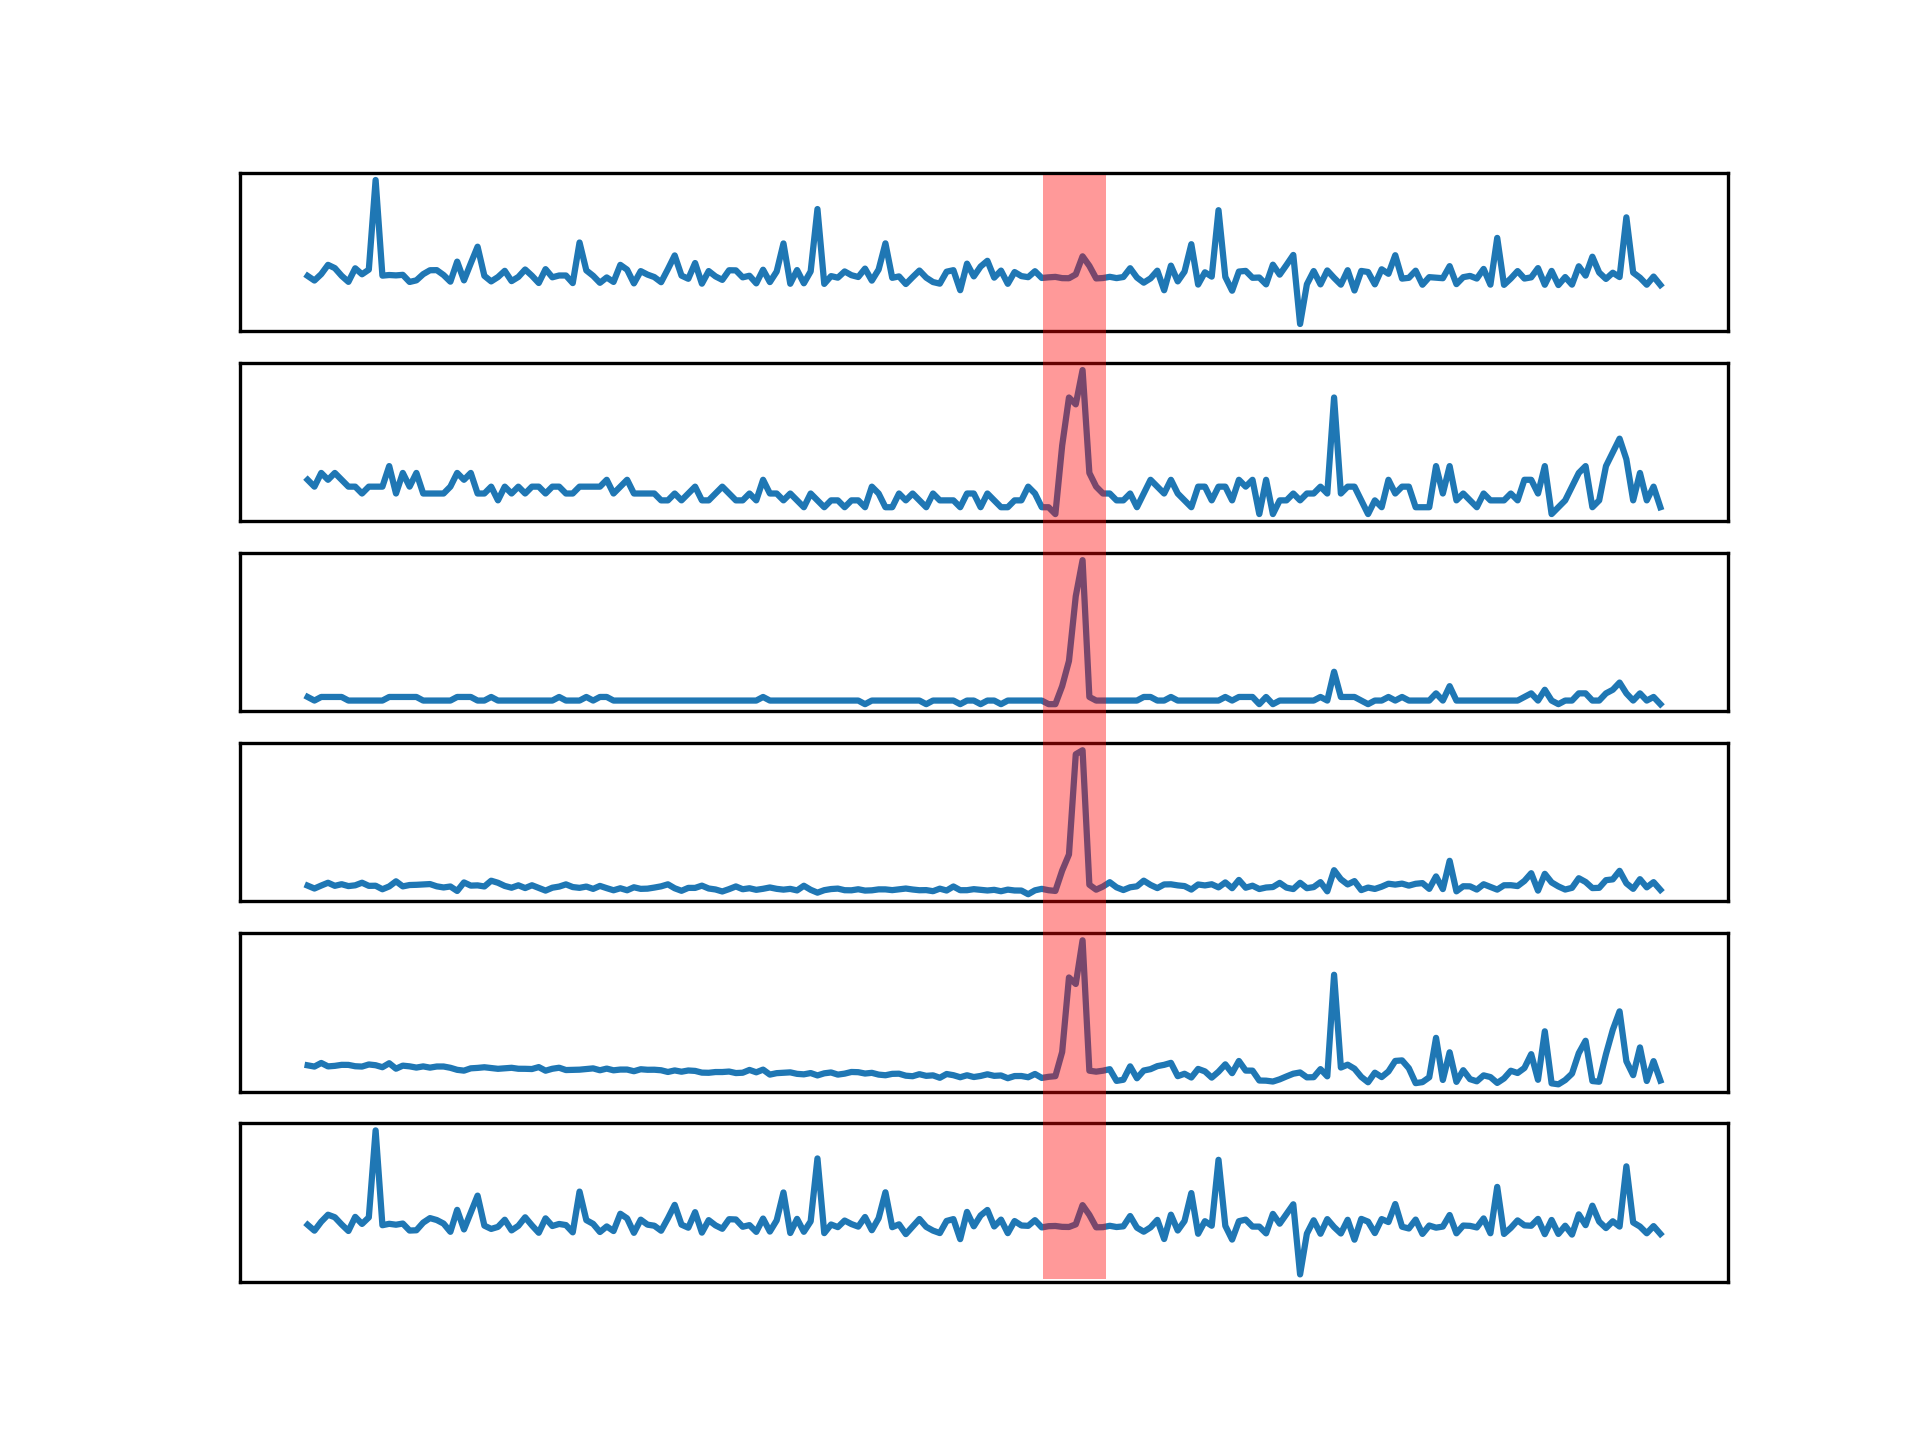
\includegraphics[width=\textwidth]{another_anomaly_example.png}
  \caption{多维时间序列数据中的一个异常示例,数据采集自SMD\cite{su2019robust}数据集}
  \label{fig:anomaly_example}
\end{figure} 

\section{框架设计}
本文实现的基于深度学习的时间序列异常检测框架如图~\ref{fig:part1_overview}。

\begin{figure}[htbp]
    \centering
    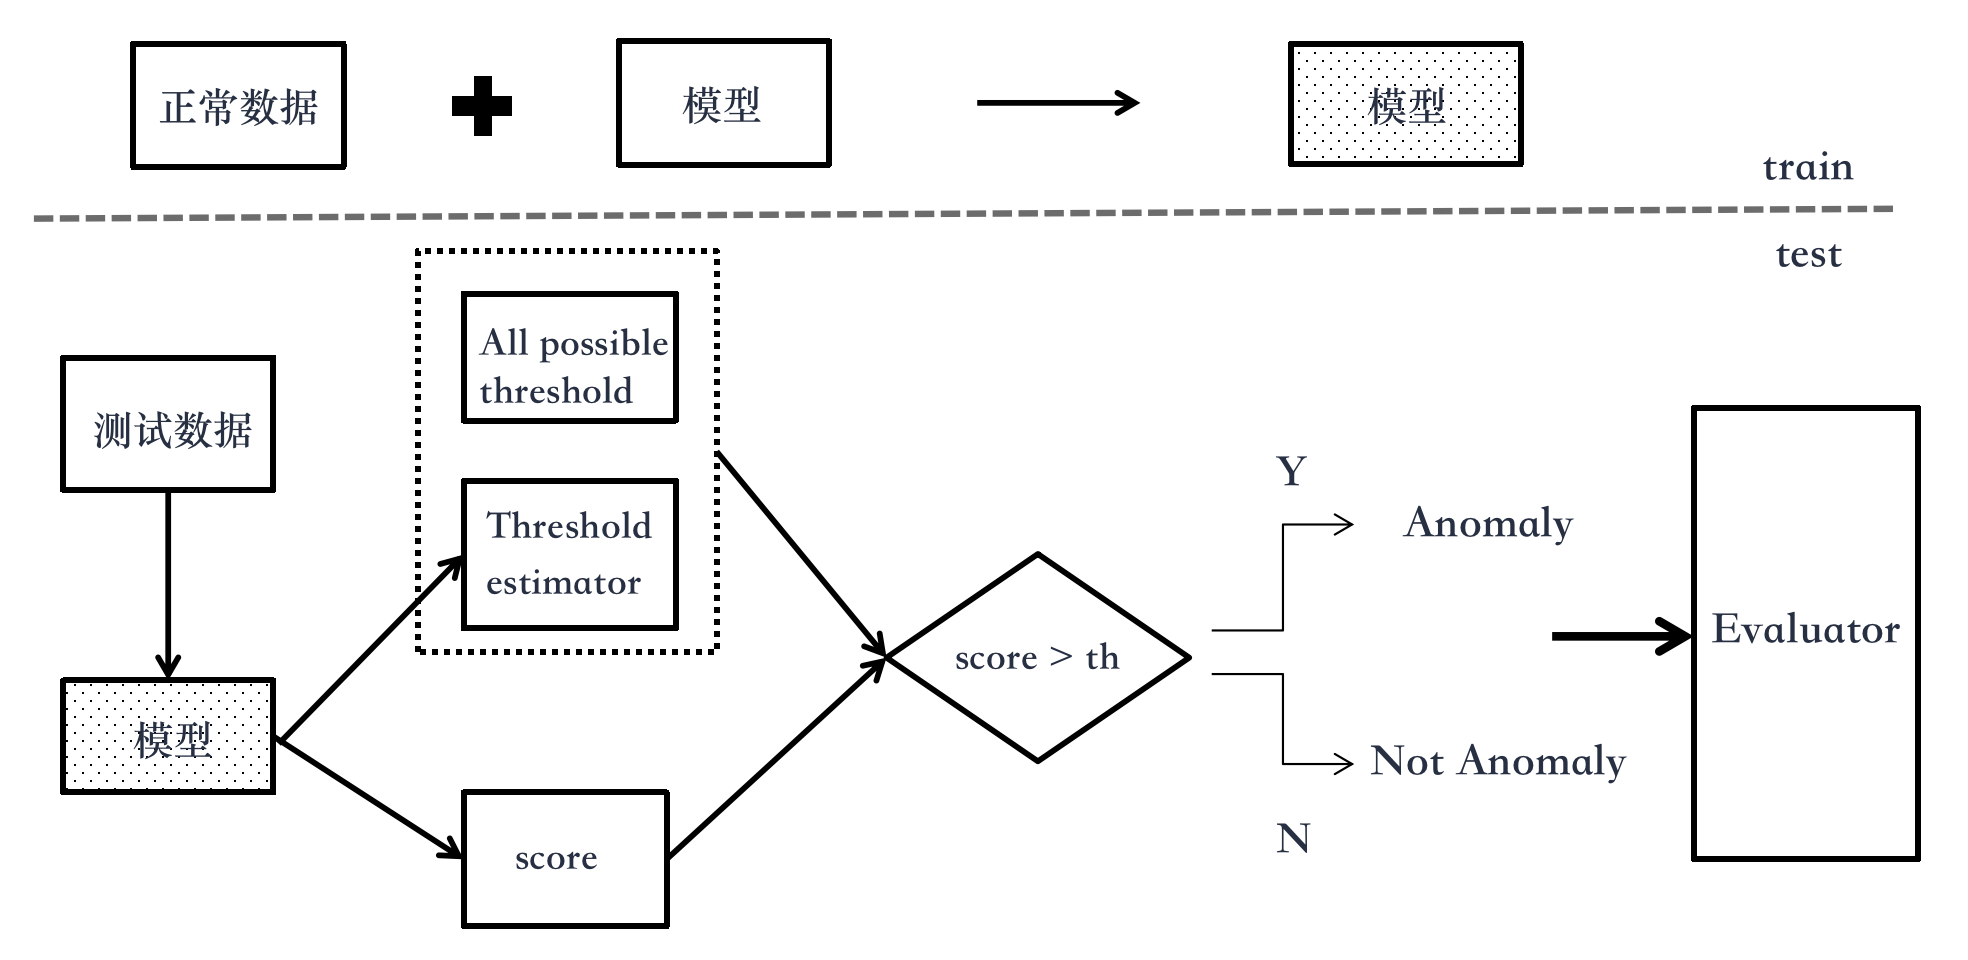
\includegraphics[width=\textwidth]{part1_overview.png}
    \caption{时间序列异常检测框架}
    \label{fig:part1_overview}
  \end{figure}

本文设计的框架分为训练和测试两个步骤。在训练时,需要先用正常数据结合某个特定的模型训练出一个适用于该数据集的模型。然后在测试时,模型对于每一时刻会输出一个非负的异常分数,表示此时的异常程度,值越大则表示越异常。由于最终输出的是一个是否是异常的0/1值,所以通常情况下还需要模型来提供一个阈值,当异常程度>给定阈值时,认为该条数据是异常,否则认为正常。为了验证与比较算法的效果本文会将预测结果送到评估模块与真实的异常标签进行结果的评估。由于阈值的确立有多种方法,每个算法适用的确立阈值的方法也不尽相同,因此本文还同时枚举所有可能的阈值对结果进行评估,选取结果最好的来衡量模型的上限\cite{xu2018unsupervised,su2019robust,DBLP:conf/ipccc/LiCP18,DBLP:conf/infocom/ChenXLPCQFW19}。

接下来分别对框架的几个关键部分进行阐述。
\section{数据集选择}
目前用来做多维时间序列数据异常检测的数据集如表~\ref{tab:dataset}所示:

\begin{table}[htbp]
  \centering
  \begin{tabular}{lcccc}
    \toprule
    名称 & 类型 & 单点数量 & 指标数量  & 指标名称 \\
    \midrule
    SMD\cite{su2019robust} & 服务器数据 & 28 & 38 & CPU利用率,网络吞吐量等\\
    SMAP\cite{DBLP:conf/kdd/HundmanCLCS18} & \multirow{2}{*}{飞船监测数据} & 55 & 25 & \multirow{2}{*}{辐射,温度,功率等}\\
    MSL\cite{DBLP:conf/kdd/HundmanCLCS18} &  & 27 & 55 &  \\
    Robot\cite{park2018multimodal} & 机器人传感数据 & \approx 39 & 17 & 运动,视觉,听觉,触觉等\\
    Engine\cite{malhotra2016lstm} &工业机器监测数据 & - & 12 & 加速器,扭矩,温度等\\
    \bottomrule
  \end{tabular}
  \caption{多元时间序列数据异常检测的数据集\cite{su2019robust}}
  \label{tab:dataset}
\end{table}

考虑到场景的类似性,本文选择了在SMD\cite{su2019robust}数据集上完成实验。其是从国内某互联网公司的服务器上采集的真实数据进行脱敏处理后的结果。测量了28台机器上的38个指标长达5周的结果,也就是$M=38$,每个机器上都采集了等间隔的超过40000个时间点的数据,然后将数据平均分为了两部分,一部分全是正常数据$x_{train}$,其中不包含异常,而另一部分则包含异常$x_{test}$并且提供了标记$y_{test}$用来测试。

\section{模型选择模块}
\label{sec:model:select}
在算法的选择方面,本文实现了两部分的算法,一部分是复现一些经典的算法,另一部分则是对已有算法进行一些修改来适应于当前的问题。
\subsection{复现算法}
本文复现了一些经典的异常检测算法,主要包含两类,一类是用于单点异常检测的算法,即将每个时间点的数据当成独立不相关的数据进行检测,也就是将这些模型看做一个函数的话,就是$y_t = \Phi (x_t)$,包含AutoEncoder、Variational AutoEncoder\cite{an2015variational}、Deep SVDD\cite{ruff2018deep}、DAGMM\cite{zong2018deep}、ConAD\cite{nguyen2018anomaly}等;另一类则是时间序列数据的异常检测方法,即判断每一时刻的状态时不仅要看当前的指标监测值,还要看之前一段时间的数据,不妨令这段时间长度为$T$,则$y_t = \Phi(x_{t-T},x_{t-T+1},\dots,x_{t})$,具体包括LSTM、LSTM-ED\cite{malhotra2016lstm}。

其中除了ConAD都在~\ref{sec:intro:time}节有所介绍,而ConAD是Nguyen等人\cite{nguyen2018anomaly}提出的用多假设方法来做异常检测的一个方法,其将Rupprechtd等人\cite{DBLP:conf/iccv/RupprechtLDB17}提出的多假设模型应用到自编码器上,如图~\ref{fig:mh}所示将自编码器的输出设置为多个。原始的自编码器的loss计算方式为$\mathcal{L}(\hat{x},x)$,其中$\mathcal{L}$可以是任意一个loss函数;而多假设的自编码器的loss计算方式则为$\min_{1\leq i\leq k}\mathcal{L}(\hat{x_i},x)$。当有一部分正常数据共享相同的潜在变量$z$时,因为整个模型共享一套参数,原先的自编码器的训练方式倾向于输出较为“模糊”的结果,即几个正常数据点的平均值,所以重构出来的数据离几个原始数据的距离都差不多,但也没有一个的重构的效果特别好,而多假设可以分工协作,每个假设专注于重构一类数据,输出一个较为“清晰”的结果。Nguyen等人\cite{nguyen2018anomaly}再在此基础上加入了GAN\cite{DBLP:conf/nips/GoodfellowPMXWOCB14}等技术使得训练出来的多个假设尽可能不相同。原方法在图像异常检测领域上取得了较好的结果,本文将其模型架构修改适用于本文针对的单点异常检测。

\begin{figure}[htbp]
  \centering
  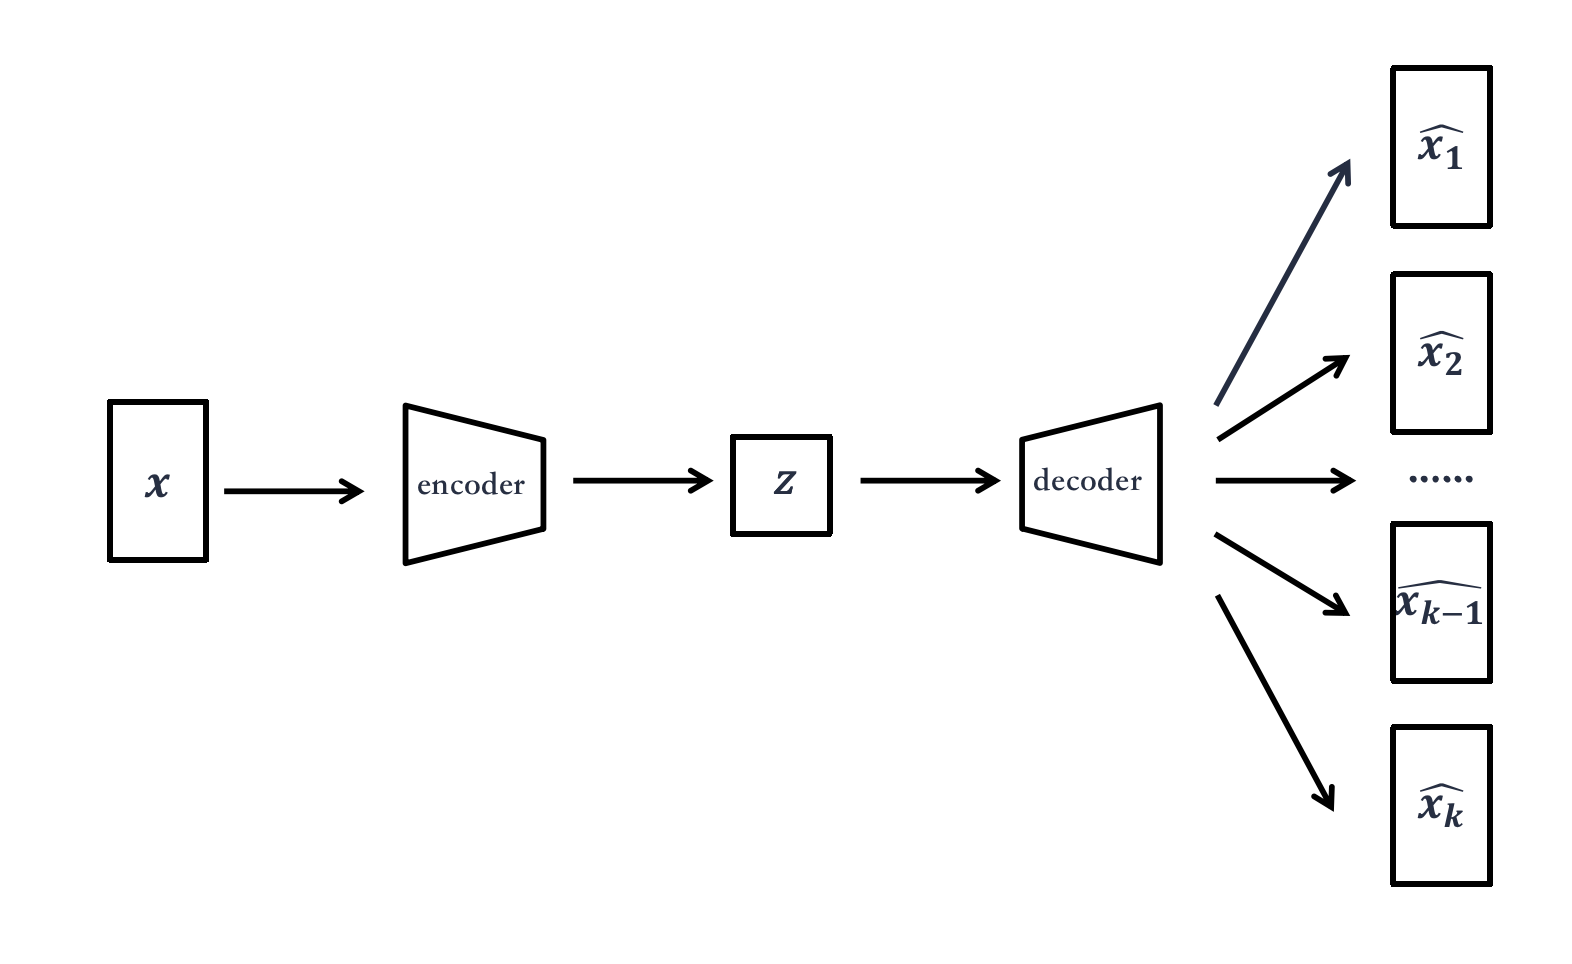
\includegraphics[width=\textwidth]{mh.png}
  \caption{多假设的自编码器}
  \label{fig:mh}
\end{figure}

\subsection{改进算法}
在已有算法的基础上,本文做出了两方面的改进。

一方面是修改已有的用于单点异常检测的算法结构来使其适应时间序列异常检测,将原来的单点方法与时序模型例如LSTM结合起来捕捉时间上的依赖信息,具体做法是将原算法中的Linear层替换成LSTM层来保留和捕捉历史信息,比方说对AutoEncoder模型的改变如图~\ref{fig:lstm_ae}所示。依据此种方法,本文还对VAE、ConAD进行修改分别得到了LSTM-VAE和LSTM-ConAD模型。

\begin{figure}[htbp]
  \begin{minipage}[t]{0.5\linewidth}
  \centering
  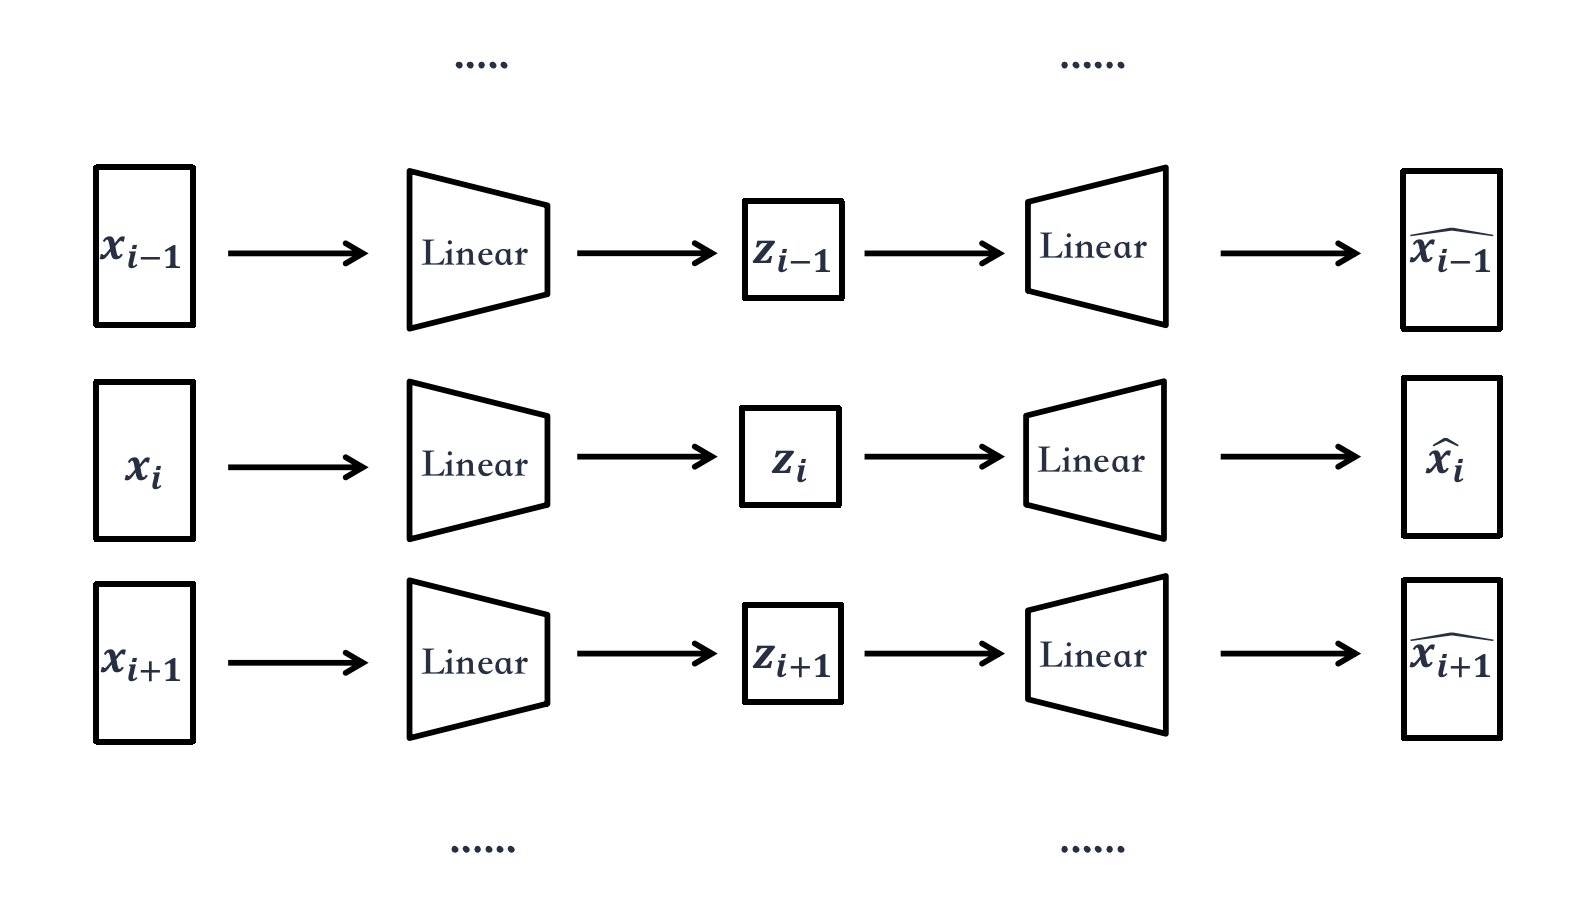
\includegraphics[width=\textwidth]{AE.png}
  \caption*{原先的AutoEncoder模型}
  \end{minipage}
  \begin{minipage}[t]{0.5\linewidth}
  \centering
  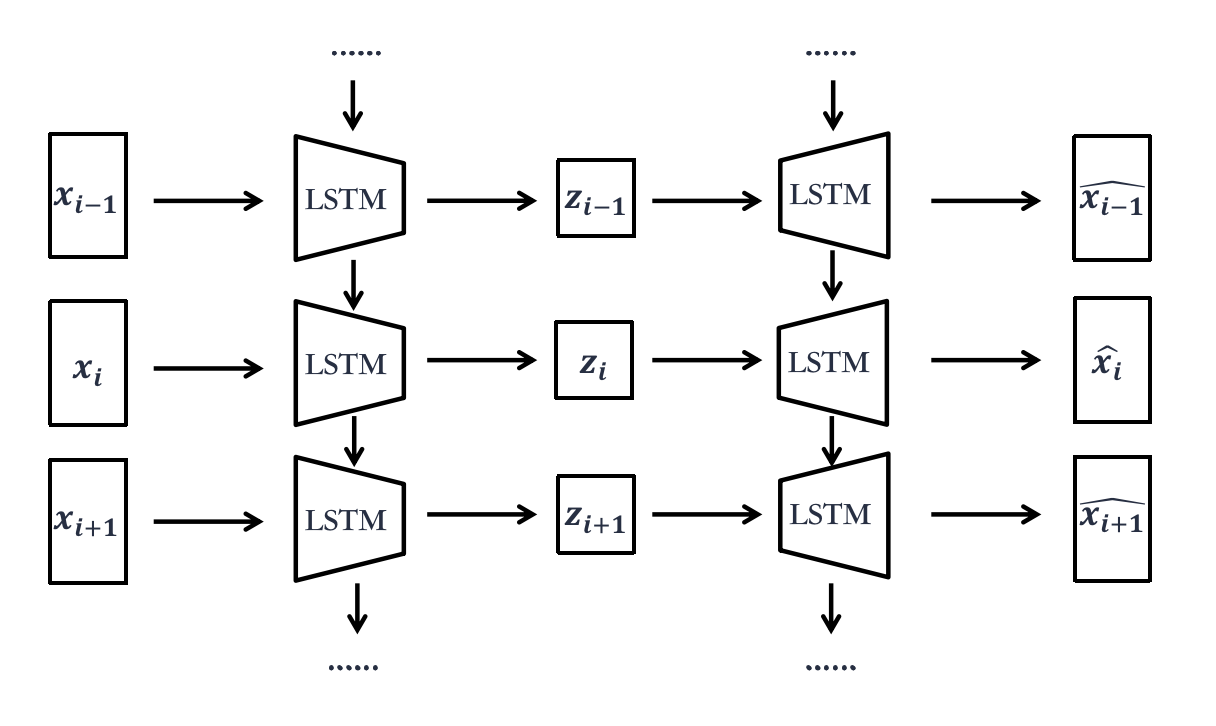
\includegraphics[width=0.95\textwidth]{LSTM_AE.png}
  \caption*{经过修改后的LSTM\_AE模型}
  \end{minipage}
  \caption{对AutoEncoder的模型修改过程}
  \label{fig:lstm_ae}
\end{figure}

另一方面是本文将LSTM的预测与AE的重构结合起来,提出了一个AE-Predictor模型,其结构如图~\ref{fig:AE-Predictor}所示。

\begin{figure}[htbp]
  \centering
  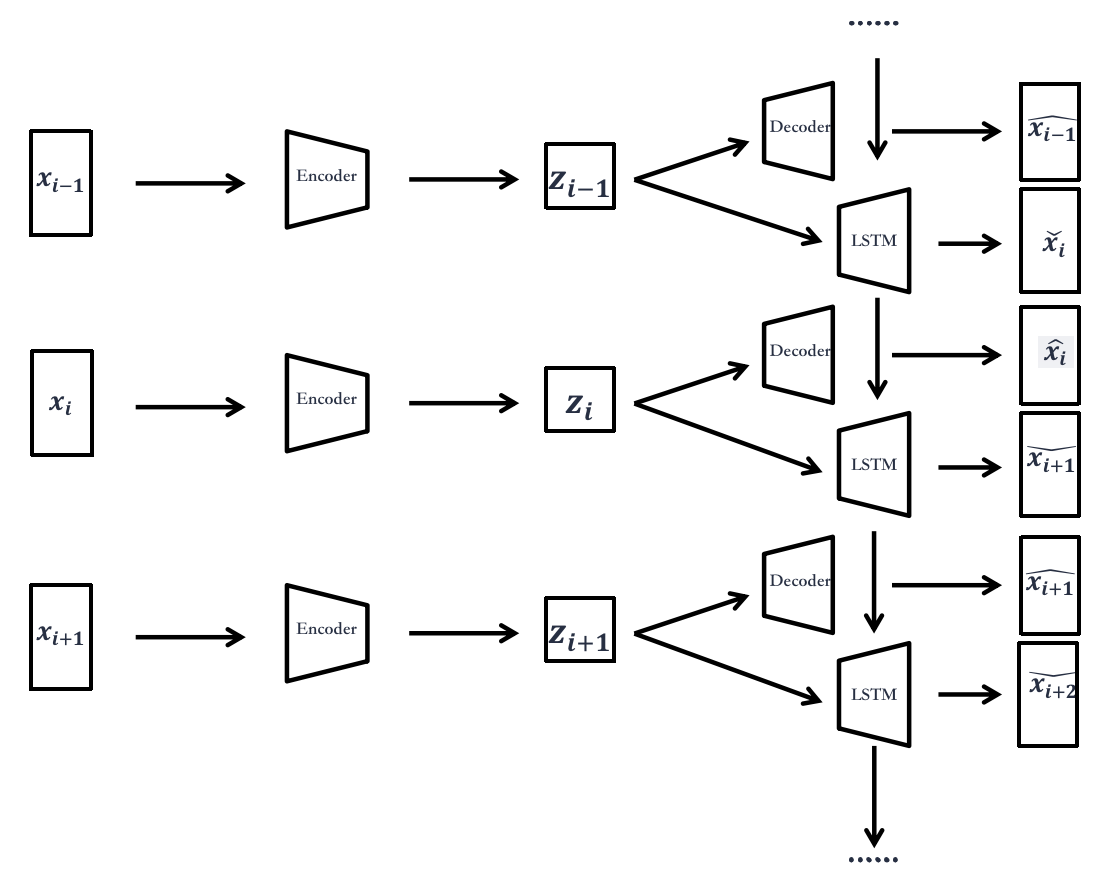
\includegraphics[width=0.7\textwidth]{AE_Predictor.png}
  \caption{AE-Predictor模型示意图}
  \label{fig:AE-Predictor}
\end{figure}

目的是要让AE学习的低维表示不仅具有重构当前数据的能力,同时低维表示序列还具有能够预测下一时刻数据的能力,也就是捕捉到时序依赖,以此达到更好的异常检测效果。训练时的loss分为两部分,重构误差和预测误差:
\begin{equation*}
  loss = \lambda \mathcal{L}(x_i,\widehat{x_{i}}) + \mathcal{L}(\widecheck{x_{i+1}},x_{i+1})
\end{equation*}

其中$\lambda$用来协调重构和预测各自所占的权重,实验中设置为1。最终将测试数据的loss作为异常分数进行输出。

\section{动态阈值选取模块}
~\ref{sec:model:select}节模型输出得到了$s = [s_1, s_2,\dots,s_N]$,其中$s_t\in \mathbb{R}^+$,$t\leq N$,要想进一步得到0/1值的$y$,需要一个模型提供的或者人为提供的阈值$threshold$来作进一步的变换:
\begin{equation*}
  y_t = \begin{cases}
    0, & s_t < threshold \cr
    1, & s_t \geq threshold
  \end{cases}
\end{equation*}

通常情况下,该阈值的确立有多种方法,一种是假设异常分数满足特定分布,例如高斯分布,求出正常数据下的异常分数的均值$\mu$和方差$\sigma$,那么异常分数超过$\mu + 3\sigma$的数据理论上不到0.3\%,那么就可以认为异常分数位于这个范围内数据是异常,但实际的异常分数很难从理论上证明符合高斯分布,通常情况下也确实不符合;还有一种比较简单的方式是假设异常是异常分数最高的那一批,通过人为设定一个分位数,例如5\%,那么在测试时就直接将最高的那5\%的数据标为异常,但这个分位数的选取也是个难题,异常的比例事先并不知道,而且,该方法需要知道整个测试集的情况才能确立阈值,意味着只能做离线的异常检测;还有一种方法是在划分得到一个验证集,在验证集上选取合适的阈值,然后基于验证集和测试集类似的假设来期待在测试集上获得较好的效果,这种方法的缺点在于还需要另一份有标数据来进行阈值的确定,在真正落地的时候难度较大。

受到\cite{siffer2017anomaly}的启发,本文使用了极值理论中的POT方法来确立异常分数的阈值,好处是无需对异常分数的分布做出任何假设,就可以较为准确、动态地确立阈值。其基本思想就是通过带有参数的GPD\footnote{Generalized Pareto Distribution,广义帕累托分布}来拟合概率分布的尾部:
\begin{equation*}
  \hat{F}_{t}(s) = P(S - t > s | S > t) \approx (1 + \frac{\gamma s}{\beta})^{-\frac{1}{\gamma}}
\end{equation*}

其中$S$是任意一个异常分数,$t$是一个较大的初始值,用来划分得到尾部区域,可以凭经验地设为正常数据的异常分数的一个较大的分位数用level表示,$\gamma$和$\beta$是GPD的形状和比例参数,是两个未知参数,可以用最大似然估计的方法估计得到$\hat{\gamma}$和$\hat{\beta}$,然后通过以下公式计算最终阈值$threshold$:
\begin{equation*}
  threshold \approx t + \frac{\hat{\beta}}{\hat{\gamma}}((\frac{qN'}{N_{t}})^{-\hat{\gamma}}-1)
\end{equation*}

其中$q$是观察到$S<threshold$的期望概率,可以凭经验确定为一个很小的数值例如$10^{-4}$,$N'$是总的数据点个数,$N_{t}$是尾部数据点的个数。

具体使用时,本文先用正常数据训练之后得到的异常分数得到一个尾部的界限即$t$,然后用最大似然估计得到一个尾部的GPD分布,同时得到一个阈值。投入使用时,每次新来一个异常分数,根据阈值将其转化成0/1值,之后判断该异常分数是否落到了尾部区域,是的话重新用最大似然估计计算GPD分布的参数使得GPD的拟合随着数据量的增加越来越准确。因为异常并不会很多,所以理论上使用最大似然估计计算的次数也不会多。设训练集上的异常分数为$s_{train}$,测试机上的异常分数为$s_{test}$,则总体过程如算法~\ref{algorithm:pot}所示。 

\begin{algorithm}
  \caption{动态确立阈值方法}
  \begin{algorithmic}[1]
      \Require $q,\ level,\ s_{train},\ s_{test}$
      \Ensure $y$
      \State $t$ \gets \ $level$th quantile of $s_{train}$
      \State $Tail$ \gets \ last $1-level$ percentile of $s_{train}$
      \State $\hat{\gamma}, \hat{\beta}$ = \Call{MaximumLikelihoodEstimation}{$Tail$}
      \State $threshold = t + \frac{\hat{\beta}}{\hat{\gamma}}((\frac{qN'}{N_{t}})^{-\hat{\gamma}}-1)$ 
      \ForAll{$s_i \in S_{test}$}
      \If{$s_i > threshold$}
      \State $y_i = 1$
      \Else \State $y_i = 0$
      \EndIf
      \State $N'$ \gets $N' + 1 $
      \If{$s_i > t$}
      \State Add $s_i$ to $Tail$
      \State $N_t$ \gets $N_t + 1$
      \State $\hat{\gamma}, \hat{\beta}$ = \Call{MaximumLikelihoodEstimation}{$Tail$}
      \State $threshold = t + \frac{\hat{\beta}}{\hat{\gamma}}((\frac{qN'}{N_{t}})^{-\hat{\gamma}}-1)$ 
      \EndIf
      \EndFor
  \end{algorithmic}
  \label{algorithm:pot}
\end{algorithm}

总体来讲几种确立阈值的方法总结如表~\ref{tab:threshold}所示。


\begin{table}[htbp]
  \centering
  \begin{tabular}{lccc}
    \toprule
    方法 & 假设 & 有标 & 在线 \\
    \midrule
    假设异常分数满足特定分布 & 强 & × & √ \\
    假设异常占一定比例 & 强 & × & × \\
    划分验证集 & 弱 & √ & √ \\
    POT & 弱 & × & √\\
    \bottomrule
   \end{tabular}
   \caption{确立阈值的方法对比}
   \label{tab:threshold}
\end{table}

\section{评价模块}
在异常检测领域,用的最多的评价指标是F\_1-Score,计算方式为
\begin{equation*}
  Precision = \frac{TP}{TP + NP}
\end{equation*}

\begin{equation*}
  Recall = \frac{TP}{TP + FN}
\end{equation*}

\begin{equation*}
  F_1-Score = 2\times \frac { Precision \times Recall}{Precision + Recall}
\end{equation*}

其中$TP$、$TN$、$FP$、$FN$分别代表true positives、true negatives、false positives和 false negatives。$Precision$描绘的是实际异常中检测出的所有异常的比例,而$Recall$描绘了所有的异常中被检测到的比例,直觉上来看,两者是对立的,只用其中一个用来评价检测器的性能是不合理的。但在单点的异常检测中,将它们结合在一起的$F_1-Score$已经被认为是公认的有效的评价方式。但对于时间序列数据的异常检测来说,这样的评价就不太准确。主要原因是因为在时间序列数据中异常的发生通常是连续的一段,如图\ref{fig:anomaly_example}所示。对于一段真正的异常而言,检测到异常的点的个数以及检测出来的位置都反映了模型效果的不同,例如一段长度为10的异常,模型$A$检测到了其中的8个,而模型$B$只检测到了1个,那么相对而言前者的效果会更好;如果模型$A$在这段异常开始的第一个位置就检测到了异常,而模型$B$直到第5个点才检测到,那么在实际投入使用时,前者的效果一定更想得到的,能够帮助工作人员更早地发现异常。之前的一些工作\cite{xu2018unsupervised}\cite{su2019robust}用了一种point-wise的方法来对算法得到的结果进行调整然后再进行评估,具体就是对于一个真实的异常而言,如果算法主要检测到了范围内的一个位置,那么整段异常就认为都被检测到。该评价方法没有考虑到检测到的点的位置和检测到的点数的影响,会造成评价指标的虚高。

基于以上考虑,本文借用了\cite{tatbul2018precision}的新型的Precision和Recall的计算方式,并根据本文针对的问题进行了一些简化和计算效率上的优化。

具体来讲首先将异常表示成区间的集合,真实的异常为$R=[R_1,R_2,\dots,R_{N_r}]$,其中每个$R_i$代表一个区间的异常,不妨认为$R_i.l$和$R_i.r$分别代表该区间的左右端点。同理$P=[P_1,P_2,\dots,P_{N_p}]$表示预测出来的异常。
\begin{equation*}
  Recall(R,P) = \frac{\sum_{i=1}^{N_r} Recall_T(R_i,P)}{N_r}
\end{equation*}

其中$Recall_T$的计算由两部分加权组成:分别考虑了存在性以及位置性。
\begin{equation*}
  Recall_T(R_i,P) = \alpha \times ExistenceReward(R_i,P) + (1-\alpha) \times OverlapReward (R_i,P)
\end{equation*}

存在性只需要判断是否存在一个检测出的异常区间当前的实际异常有交集。
\begin{equation*}
ExistenceReward(R_i,P) = \begin{cases} 1, & \ \exists \  | R_i \cap P_j|>1 \cr 0, & otherwise \end{cases}
\end{equation*}

而相交性则需要考虑重叠的位置和大小的关系,此处本文认为对于一段异常来说,越早检测到说明效果越好,因此将靠前的位置分配较大的权重,具体计算如算法~\ref{algorithm:omega1}所示。
\begin{equation*}
  OverlapReward(R_i,P) = \sum_{j=1}^{N_p}\omega(R_i,R_i\cap P_j)
\end{equation*}
\begin{algorithm}
  \caption{$\omega$ 原版计算方法\cite{tatbul2018precision}}
  \begin{algorithmic}[1]
      \Function{$\omega$}{AnomalyRange, OverlapRange}
      \State DetectValue \gets 0
      \State TotalValue \gets 0
      \State len \gets length(AnomalyRange)
      \For {i = 1  \to len}
          \State Value \gets len - i + 1
          \State TotalValue \gets TotalValue + Value
          \If {AnomalyRange[i] in OverlapRange}
              \State DetectValue \gets DetectValue + Value
          \EndIf
      \EndFor
      \State \Return $\frac{DetectValue}{TotalValue}$
      \EndFunction
  \end{algorithmic}
  \label{algorithm:omega1}
\end{algorithm}

意识到$OverlapRange$也一定是一个区间之后,可以将$\omega$的计算方式简化为算法~\ref{algorithm:omega2}:
  \begin{algorithm}
    \caption{$\omega$ 简化计算方法}
    \begin{algorithmic}[1]
        \Function{$\omega$}{AnomalyRange, OverlapRange}
        \State len \gets length(AnomalyRange)
        \State TotalValue \gets $\frac{len \times (len + 1)}{2}$
        \State l \gets OverlapRange.l - AnomalyRange.l + 1
        \State r \gets OverlapRange.r - AnomalyRange.l + 1
        \State DetectValue \gets $\frac{r \times (r+1)}{2} - \frac{(l-1) \times l}{2}$
        \State \Return $\frac{DetectValue}{TotalValue}$
        \EndFunction
    \end{algorithmic}
    \label{algorithm:omega2}
  \end{algorithm}

新型Precision的计算方式类似:

\begin{equation*}
Precision(R,P) = \frac{\sum_{i=1}^{N_p}Precision_T(R,P_i)}{N_p}
\end{equation*}

区别是$Precision_t(R,P_i)$的计算不需要考虑$ExistenceReward$,直接按照检测到的位置计算贡献即可:
\begin{equation*}
Precision_T(R,P_i) = \sum_{j=1}^{N_r}\omega(P_i,P_i\cap R_j)
\end{equation*}

  该评价方式虽然考虑的全面,但是随之而来的就是计算代价很大,复杂度为$O(N_r\times N_p)$。当需要计算所有阈值的结果并选取最好的时候,考虑阈值按从大到小枚举所有可能的$N$个,最坏情况下的$N_p$序列为$\{1,2,3,\dots,\frac{N}{2},\frac{N}{2}-1,\frac{N}{2}-2,\dots,1\}$,则总的计算复杂度为$O(N_r\times N^2)$。

  \begin{algorithm}
  \caption{朴素的Best F1-Score计算方式}
  \begin{algorithmic}[1]
    \Function {computeBestF1Score}{R,S}
    \State bestF1Score = 0
    \ForAll {$s \in S$}
    \State P \gets convertTo01ByThreshold(S,s)
    \State bestF1Score \gets max(bestF1Score, computeF1Score(R,P))
    \EndFor
    \State \Return bestF1Score
    \EndFunction
  \end{algorithmic}
  \end{algorithm}


  本文考虑一种新的增量计算的方式,每次将阈值下调时,考虑只有一个位置$i$的预测结果从0变成了1,那么有可能有三种情况:
  \begin{enumerate}
    \item 这一个位置形成了一个新的异常区间,也就是$i-1$和$i+1$都是不存在或者为0的状态
    \item 这个位置拓宽了相邻的区间,也就是$i-1$或者$i+1$中有且只有一个位置已经被预测为1
    \item 这个位置将左右两个区间连成了一个区间,也就是$i-1$与$i+1$都存在且被预测为异常
  \end{enumerate}

  如果能够以一个较低的复杂度支持动态的在$P$中增加、减少一个异常区间同时计算$Precision$和$Recall$的值,那么就能高效的求解$Best F1-Score$。具体来讲,本文通过并查集的方式来快速维护$P$,并且用记录中间变量的方式来记录计算过程中的中间状态来实现增量的更新。具体的算法过程如下:

  \begin{breakablealgorithm}
    \caption{高效的Best F1-Score计算方式}
    \begin{algorithmic}[1]
      \State $rangeReward \gets [0] \times N_r$
      \State $rangeOverlapCount \gets [0] \times N_r$
      \State $predict \gets [0] \times N$
      \State $Recall \gets 0$
      \State $Precision \gets 0$

      \State

      \Function {computeBestF1Score}{R,S}
      \State bestF1Score = 0
      \State S \gets sorted(S) in descending order
      \ForAll {$S_i \in S$}
      \State $predict_i = 1$
      \If { $i + 1 < n\ and\ predict_{i+1} = 1$}
          \State \Call{dropPredictRange}{\Call{GetRange}{i + 1}}
          \State \Call{union}{i, i + 1}
      \EndIf
      \If {$i - 1 \geq 0\ and\ predict_{i-1} = 1$}:
          \State \Call{dropPredictRange}{\Call{GetRange}{i - 1}}
          \State \Call{union}{i, i - 1}
      \EndIf
      \State \Call{addPredictRange}{\Call{GetRange}{i}}
      \State $bestF1Score \gets max(bestF1Score, 2\times\frac{Precision \times Recall}{Precision + Recall})$
      \EndFor
      \State \Return bestF1Score
      \EndFunction
      
      \State

      \Function {addPredictRange}{p}
      \State Recall \gets 0
      \ForAll{$R_i \in R$}
            \State $rangeReward_i \gets rangeReward_i + \omega(R_i,R_i \cap p)$
            \State $overlapCount_i \gets overlapCount_i +  |R_i\cap p|$
            \If {$overlapCount_i > 0$}
              \State existReward = 1
            \Else
              \State existReward = 0
            \EndIf
            \State $overlapReward \gets rangeReward_i$
            \State $Recall \gets Recall + \alpha \times existReward + (1-\alpha) \times overlapReward$
      \EndFor
      \State $Recall = \frac{Recall}{N_r}$

      \State

      \State $reward \gets 0$
      \ForAll{$R_i \in R$}
            \State $reward \gets reward  + \omega(p, p \cap R_i)$
      \EndFor
      \State $Precision \gets \frac{Precision \times N_p + reward}{N_p + 1}$
      \State $N_p \gets N_p + 1$
      \EndFunction

      \State

      \Function {dropPredictRange}{p}
      \State Recall \gets 0
      \ForAll $R_i \in R$
            \State $rangeReward_i \gets rangeReward_i - \omega(R_i,R_i \cap p)$
            \State $overlapCount_i \gets overlapCount_i - |R_i\cap p|$
            \If {$overlapCount_i > 0$}
              \State $existReward = 1$
            \Else
              \State $existReward = 0$
            \EndIf
            \State $overlapReward \gets rangeReward_i$
            \State $Recall \gets Recall +  \alpha \times existReward + (1-\alpha) \times overlapReward$
      \EndFor

      \State

      \State $Recall \gets \frac{Recall}{N_r}$

      \State $reward \gets 0$
      \ForAll $R_i \in R$
            \State $reward \gets reward + \omega(p, p \cap R_i)$
      \EndFor
      \State $Precision \gets \frac{Precision \times N_p - reward}{N_p - 1}$
      \State $N_p \gets N_p - 1$
      \EndFunction
    \end{algorithmic}
  \end{breakablealgorithm}

  其中GetRange和Union是通过并查集来实现记录和维护某个位置所属的区间以及该区间的左右端点,算法中不再赘述。容易得知这样的计算复杂度为$O((N_r + \alpha(N))\times N)$,其中$\alpha(N)$是Ackerman函数的某个反函数,在很大一个范围内(超过$10^{80}$)可以认为是不大于4的一个常数,所以可以认为复杂度是较原先下降了一个数量级,实测原先需要4小时的计算仅需3秒就可以得出结果。
\section{实验结果与分析}
本章先对所有算法在所有阈值下的最好结果进行分析,再评估用POT方法确立阈值对结果造成的影响及其可用性,然后对比一下传统基于点的异常检测模型与时序模型结合后与原模型的效果,最对各个算法的效率进行比较。
\subsection{最好结果}
表~\ref{tab:best}为各个算法在枚举所有阈值之后得到的最好的评估结果,其中Random是随机将当前时刻分为正常或异常,OmniAnomaly是\cite{su2019robust}中提出的模型,在本文的框架内并没有实现,本文使用其公开的源代码进行了异常检测的结果获取然后放到本文的评估模块中进行评估,方便参考。
\begin{table}[htbp]
  \centering
\begin{tabular}{lccc}
  \toprule
          algorithm &  F1-Score &    Recall &  Precision \\
  \midrule
   LSTM-VAE &  0.779323 &  0.708920 &   0.865252 \\
        VAE &  0.768701 &  0.718729 &   0.826141 \\
     LSTM &  0.740222 &  0.712757 &   0.769889 \\
            LSTM-AE &  0.736745 &  0.694566 &   0.784377 \\
       AE-Preditor &  0.723190 &  0.690104 &   0.759609 \\
                 AE &  0.715418 &  0.687829 &   0.745311 \\
                 OmniAnomaly &  0.708538 &  0.662548 &   0.761388 \\
         LSTM-ConAD &  0.666084 &  0.648798 &   0.684316 \\
              ConAD &  0.655414 &  0.613009 &   0.704121 \\
          Deep SVDD &  0.585766 &  0.606182 &   0.566680 \\
            LSTM-ED &  0.582350 &  0.567344 &   0.598172 \\
              DAGMM &  0.568452 &  0.721212 &   0.469093 \\
             Random &  0.177244 &  0.813319 &   0.099459 \\
  \bottomrule
  \end{tabular}
  \caption{各个算法的枚举所有阈值选取最好的评估结果}
  \label{tab:best}
\end{table}

从表中可以看出:
\begin{itemize}
  \item 重构和预测的方法都取得了不错的效果,这其中又属将重构和预测结合起来的LSTM-VAE表现最好;
  \item ConAD模型表现并不佳,很可能是数据分布并不符合多假设分布,所以直接套用效果并不好;
  \item OmniAnomaly在自己的评价标准中是最好的,但在本文的框架中表现并不突出。从方法上来看,本文偏向于认为本文的评价方式更有说服力;
  \item 本文提出的AE-Predictor比AE的结果稍好,但仍然不如纯用LSTM的结果,可见其能捕捉到的时序特征有限;
  \item 不论是VAE和AE,还是LSTM-VAE和LSTM-AE相比较,前者的效果都要好于后者,可见用于做异常检测时,VAE的重构概率要比AE的重构误差更合理。
\end{itemize}
\subsection{POT结果}
表\ref{tab:POT}是各个方式使用POT的方法确立阈值之后评估得到的结果,从中不难看出,所有算法的效果都受到了不小的影响,可见POT算法得到的结果距离模型的上限还有一定的距离。不过总体来讲,模型的上限越高,POT算法得到的结果也越好。

\begin{table}[htbp]
  \centering
  \begin{tabular}{lccc}
    \toprule
            algorithm &  F1-Score &    Recall &  Precision \\
    \midrule
          VAE &  0.612505 &  0.647518 &   0.581085 \\
        LSTM &  0.600829 &  0.642604 &   0.564153 \\
                   AE &  0.590449 &  0.624056 &   0.560277 \\
          OmniAnomaly &  0.580469 &  0.780431 &   0.462076 \\
          LSTM-VAE &  0.561089 &  0.618607  & 0.513357 \\
         AE-Predictor &  0.554562 &  0.671442 &   0.472341 \\
             LSTM-AE &  0.551305 &  0.541161 &   0.561837 \\
                ConAD &  0.468980 &  0.357720 &   0.680692 \\
            Deep SVDD &  0.447898 &  0.598041 &   0.358016 \\
              LSTM-ED &  0.425158 &  0.374871 &   0.491028 \\
           LSTM-ConAD &  0.418753 &  0.346240 &   0.529684 \\
               Random &  0.169029 &  0.212759 &   0.140210 \\
    \bottomrule
    \end{tabular}
    \caption{各个算法的由POT确立阈值之后评估的结果}
    \label{tab:POT}
\end{table}

另一方面,本文在使用POT算法的时候需要指定$q$和$level$(作为初始化阈值的分位数)在使用时发现$q$和$level$的指定将极大的影响到最终的结果评定,拿在训练LSTM-VAE时举例,本文尝试了多种$q$和$level$的组合评价结果如表~\ref{tab:pot-lstm-vae}所示,所选$q$和$level$其实都在可接受范围内,但得到的F1-Score可以说方差非常大,而且最大差距有0.3581。可见POT方法虽然理论上具有一定的优越性,但在实际使用上,受限于对参数$q$和$level$的敏感性,在落地上还是有一定的困难。

\begin{table}[htbp]
  \centering
  \begin{tabular}{lccccc}
    \toprule
      \diagbox{q}{level} &     0.00005 &    0.0001 &    0.0005 &     0.001 &     0.005 \\
    \midrule
     0.9500 &  0.426536 &  0.417596 &  0.416071 &  0.406086 &  0.400018 \\
     0.9800 &  0.426830 &  0.446301 &  0.453475 &  0.450445 &  0.517225 \\
     0.9900 &  0.379479 &  0.410506 &  0.428053 &  0.435433 &  0.508593 \\
     0.9950 &  0.326792 &  0.334594 &  0.359302 &  0.444482 &  0.494093 \\
     0.9990 &  0.278916 &  0.304195 &  0.542905 &  0.553386 &  0.388911 \\
     0.9995 &  0.381923 &  0.443832 &  0.561089 &  0.451752 &  0.357804 \\
     0.9999 &  0.365430 &  0.533608 &  0.291709 &  0.300287 &  0.202976 \\
    \bottomrule
    \end{tabular}
    \caption{$q$和$level$取值对结果的影响}
    \label{tab:pot-lstm-vae}
\end{table}

\subsection{单点异常检测方法与时序模型结合后与原模型对比}
表~\ref{tab:lstm-diff}展示了单点的异常检测模型与结合了时序模型LSTM之后的结果与原先结果的差异,均是在best条件下。

\begin{table}[htbp]
  \centering
  \begin{tabular}{lcccc}
    \toprule
      {} &     AE &    VAE &    ConAD \\
    \midrule
     原模型 & 0.715418 & 0.768701 & 0.655414  \\
     结合LSTM之后 & 0.736745 & 0.779323 & 0.666084 \\
    \bottomrule
    \end{tabular}
    \caption{单点异常检测模型结合时序模型后模型效果的变化}
    \label{tab:lstm-diff}

\end{table}

可以看出原来用于单点异常检测的算法在与LSTM模型结合后检测效果都有了些许的提升,证明LSTM捕获时间依赖的能力确实能够帮助算法提升性能。

\subsection{效率}
图~\ref{fig:train:time}是所有算法的训练时间箱型图,可以看出
\begin{enumerate}
  \item 结合了LSTM的模型训练所花的时间普遍高于其他算法;
  \item ConAD因为模型十分复杂、要训练多个假设,训练时间也偏长;
  \item Deep SVDD因为模型结构较为简单、而DAGMM因为算法原因需要选取非常大的batch size(实验中设置为1024)因此训练速度很快。
\end{enumerate}

\begin{figure}[htbp]
  \centering
  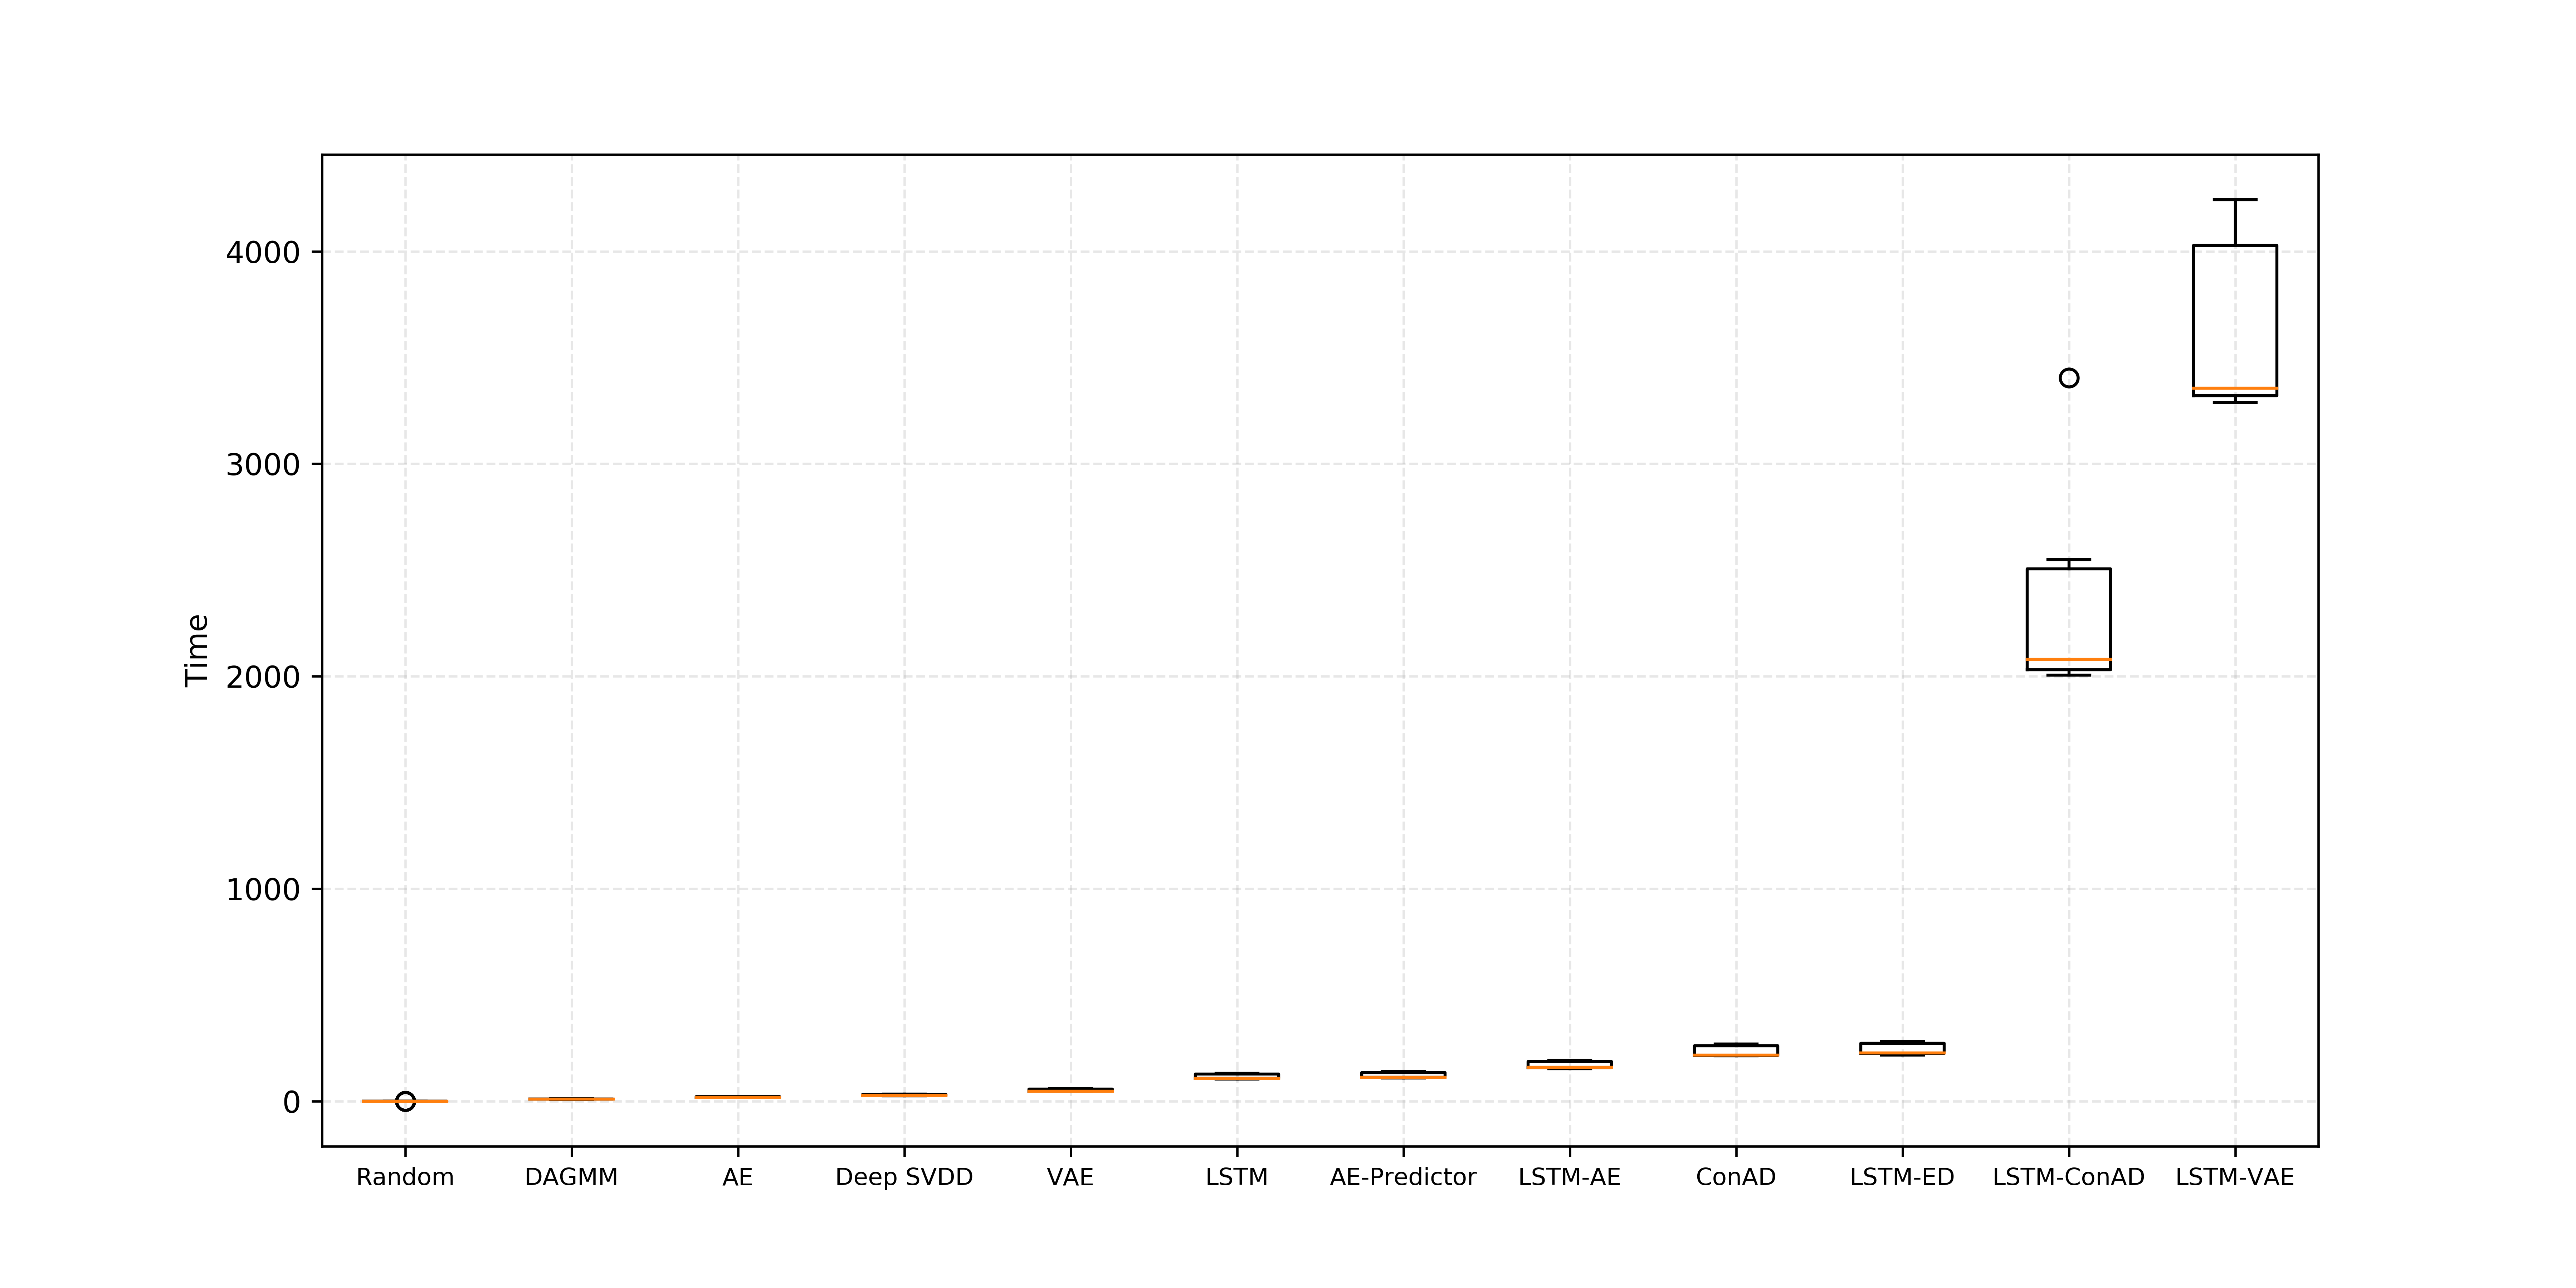
\includegraphics[width=\textwidth]{train_time.png}
  \caption{训练时间}
  \label{fig:train:time}
\end{figure}

图~\ref{fig:test:time}是所有算法的检测时间箱型图,可以看到LSTM-VAE因为使用了时序模型LSTM以及重构概率的计算要采样多次取平均,所以检测时间最长,而ConAD和LSTM-ConAD则是因为本身模型过于复杂在检测时花费时间相对较长,其他算法在检测时花费时间差距不大。

\begin{figure}[htbp]
  \centering
  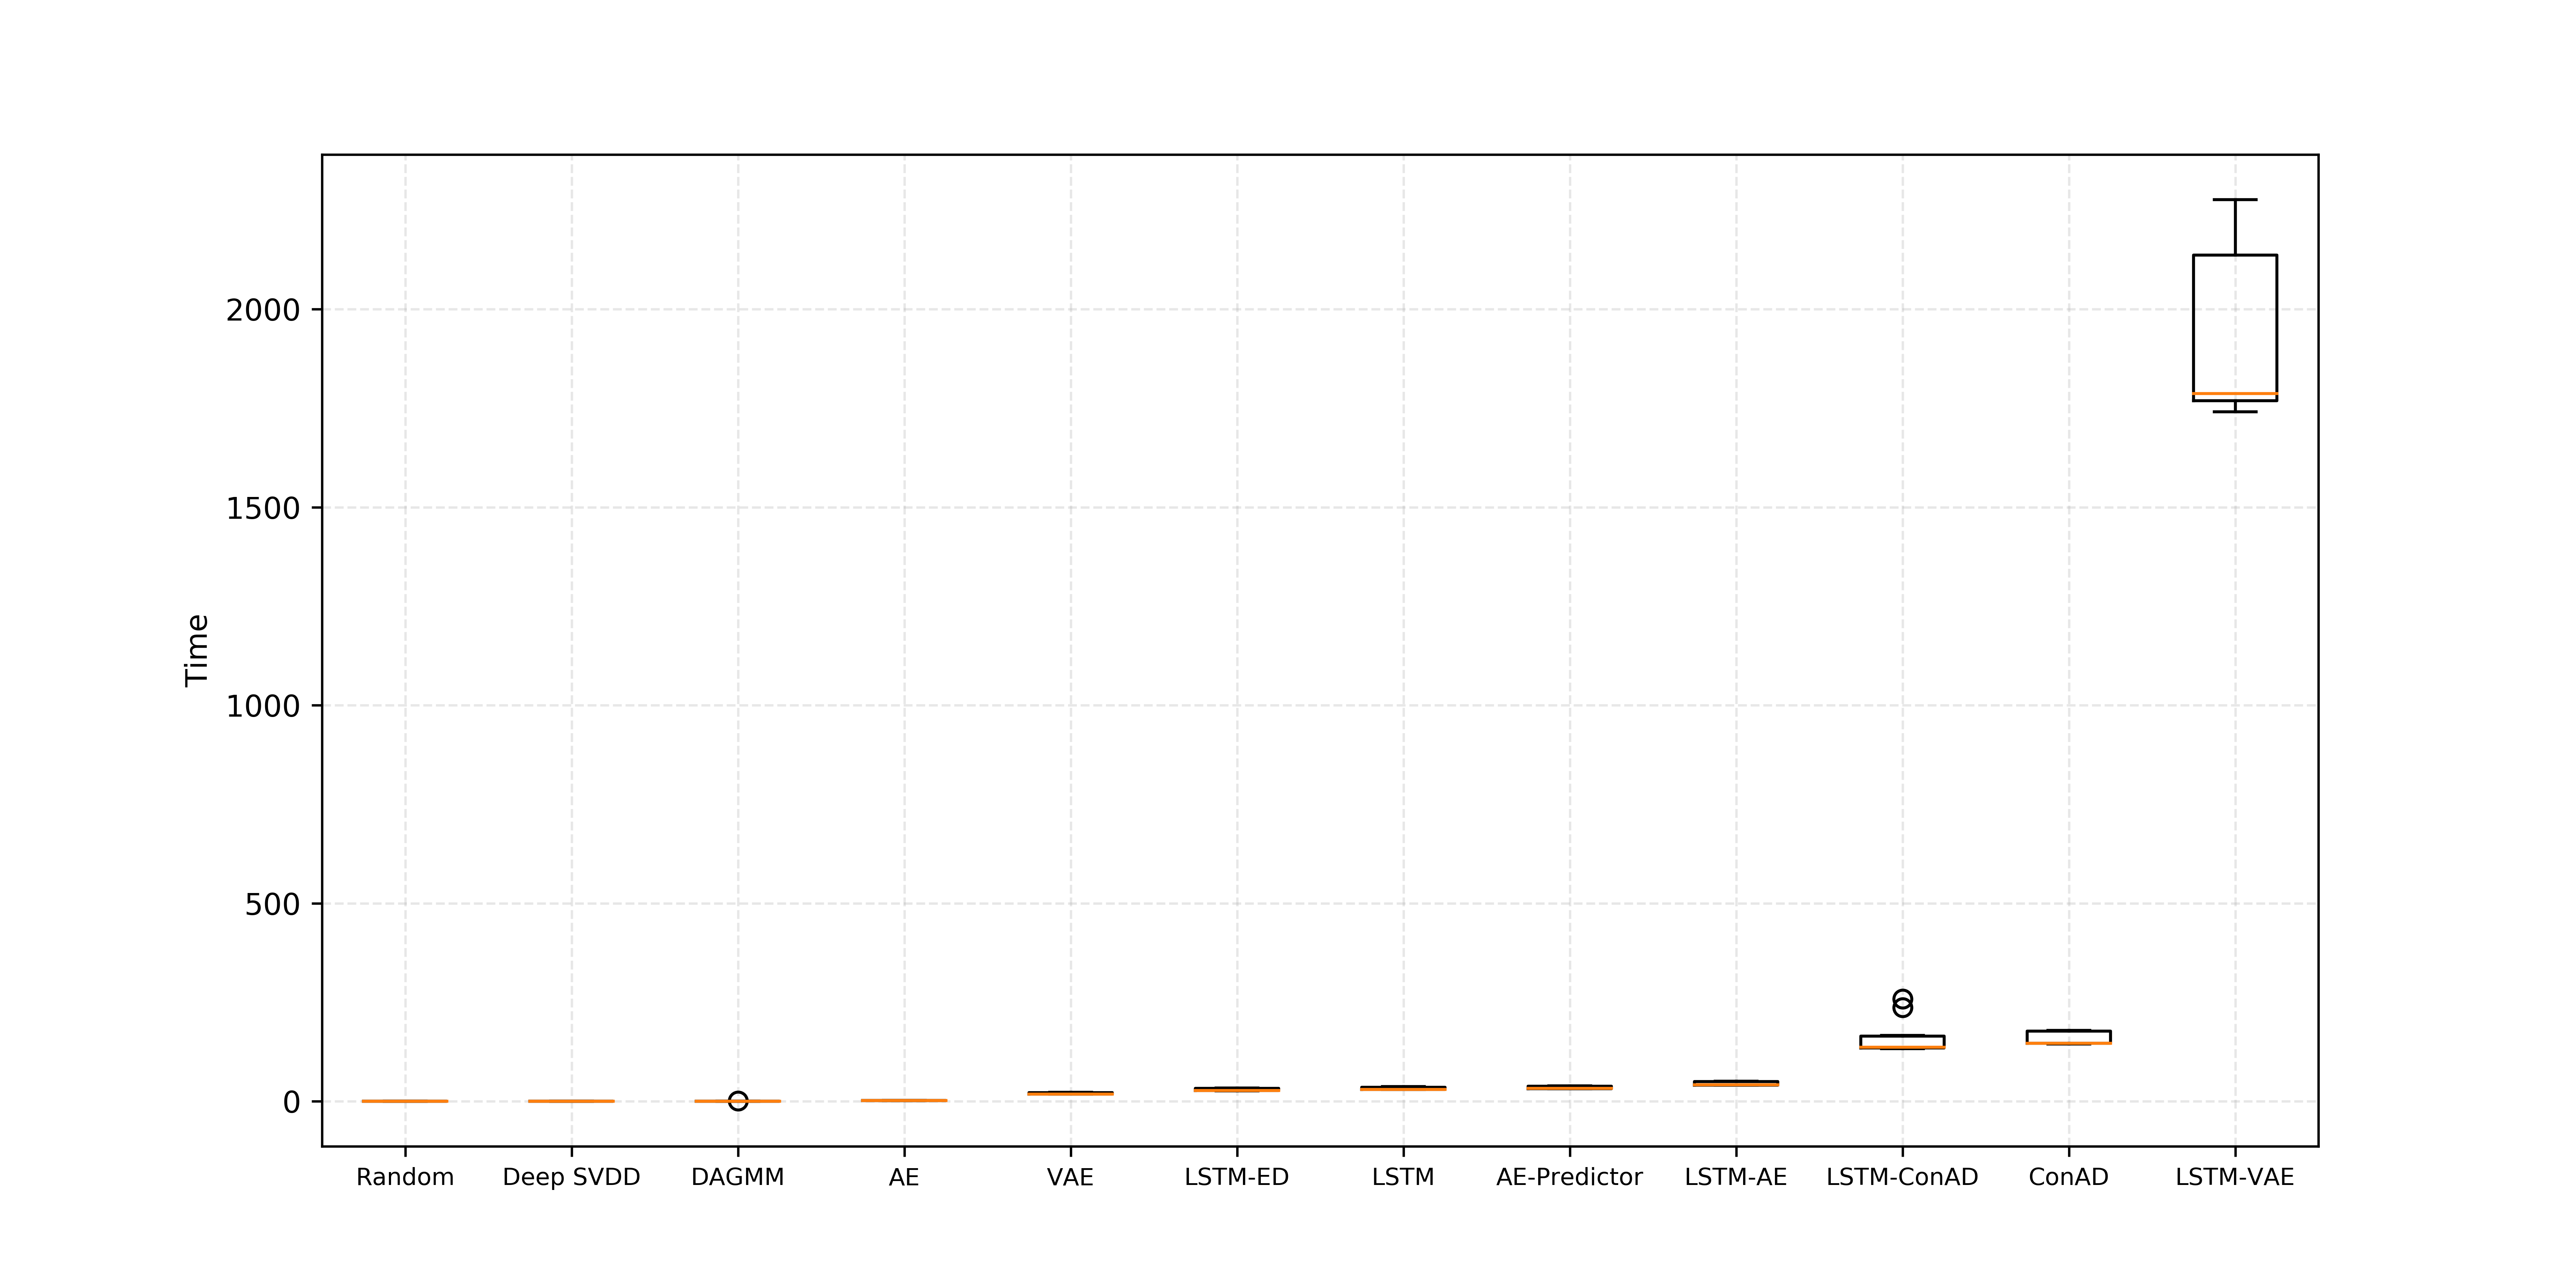
\includegraphics[width=\textwidth]{predict_time.png}
  \caption{检测时间}
  \label{fig:test:time}
\end{figure}

图~\ref{fig:pot:time}是所有算法用POT方法来确立阈值的耗时箱型图,虽然耗时的中位数很低,但是异常点很多,最坏情况下甚至达到了1000秒以上的耗时,而且稳定性较差,可以认为是由于本文采用了训练集的异常分数的分位数作为划分尾部的边界,但因为训练集都是正常的,所以其异常分数均偏低,所以这个尾部也划得比较低,导致在测试集中太多的点落到了尾部区域中,所以重新用最大似然估计估计GPD参数的次数变多,因此耗时也增长。所以该方法还是难以真正落地用到生产环境中去。

\begin{figure}[htbp]
  \centering
  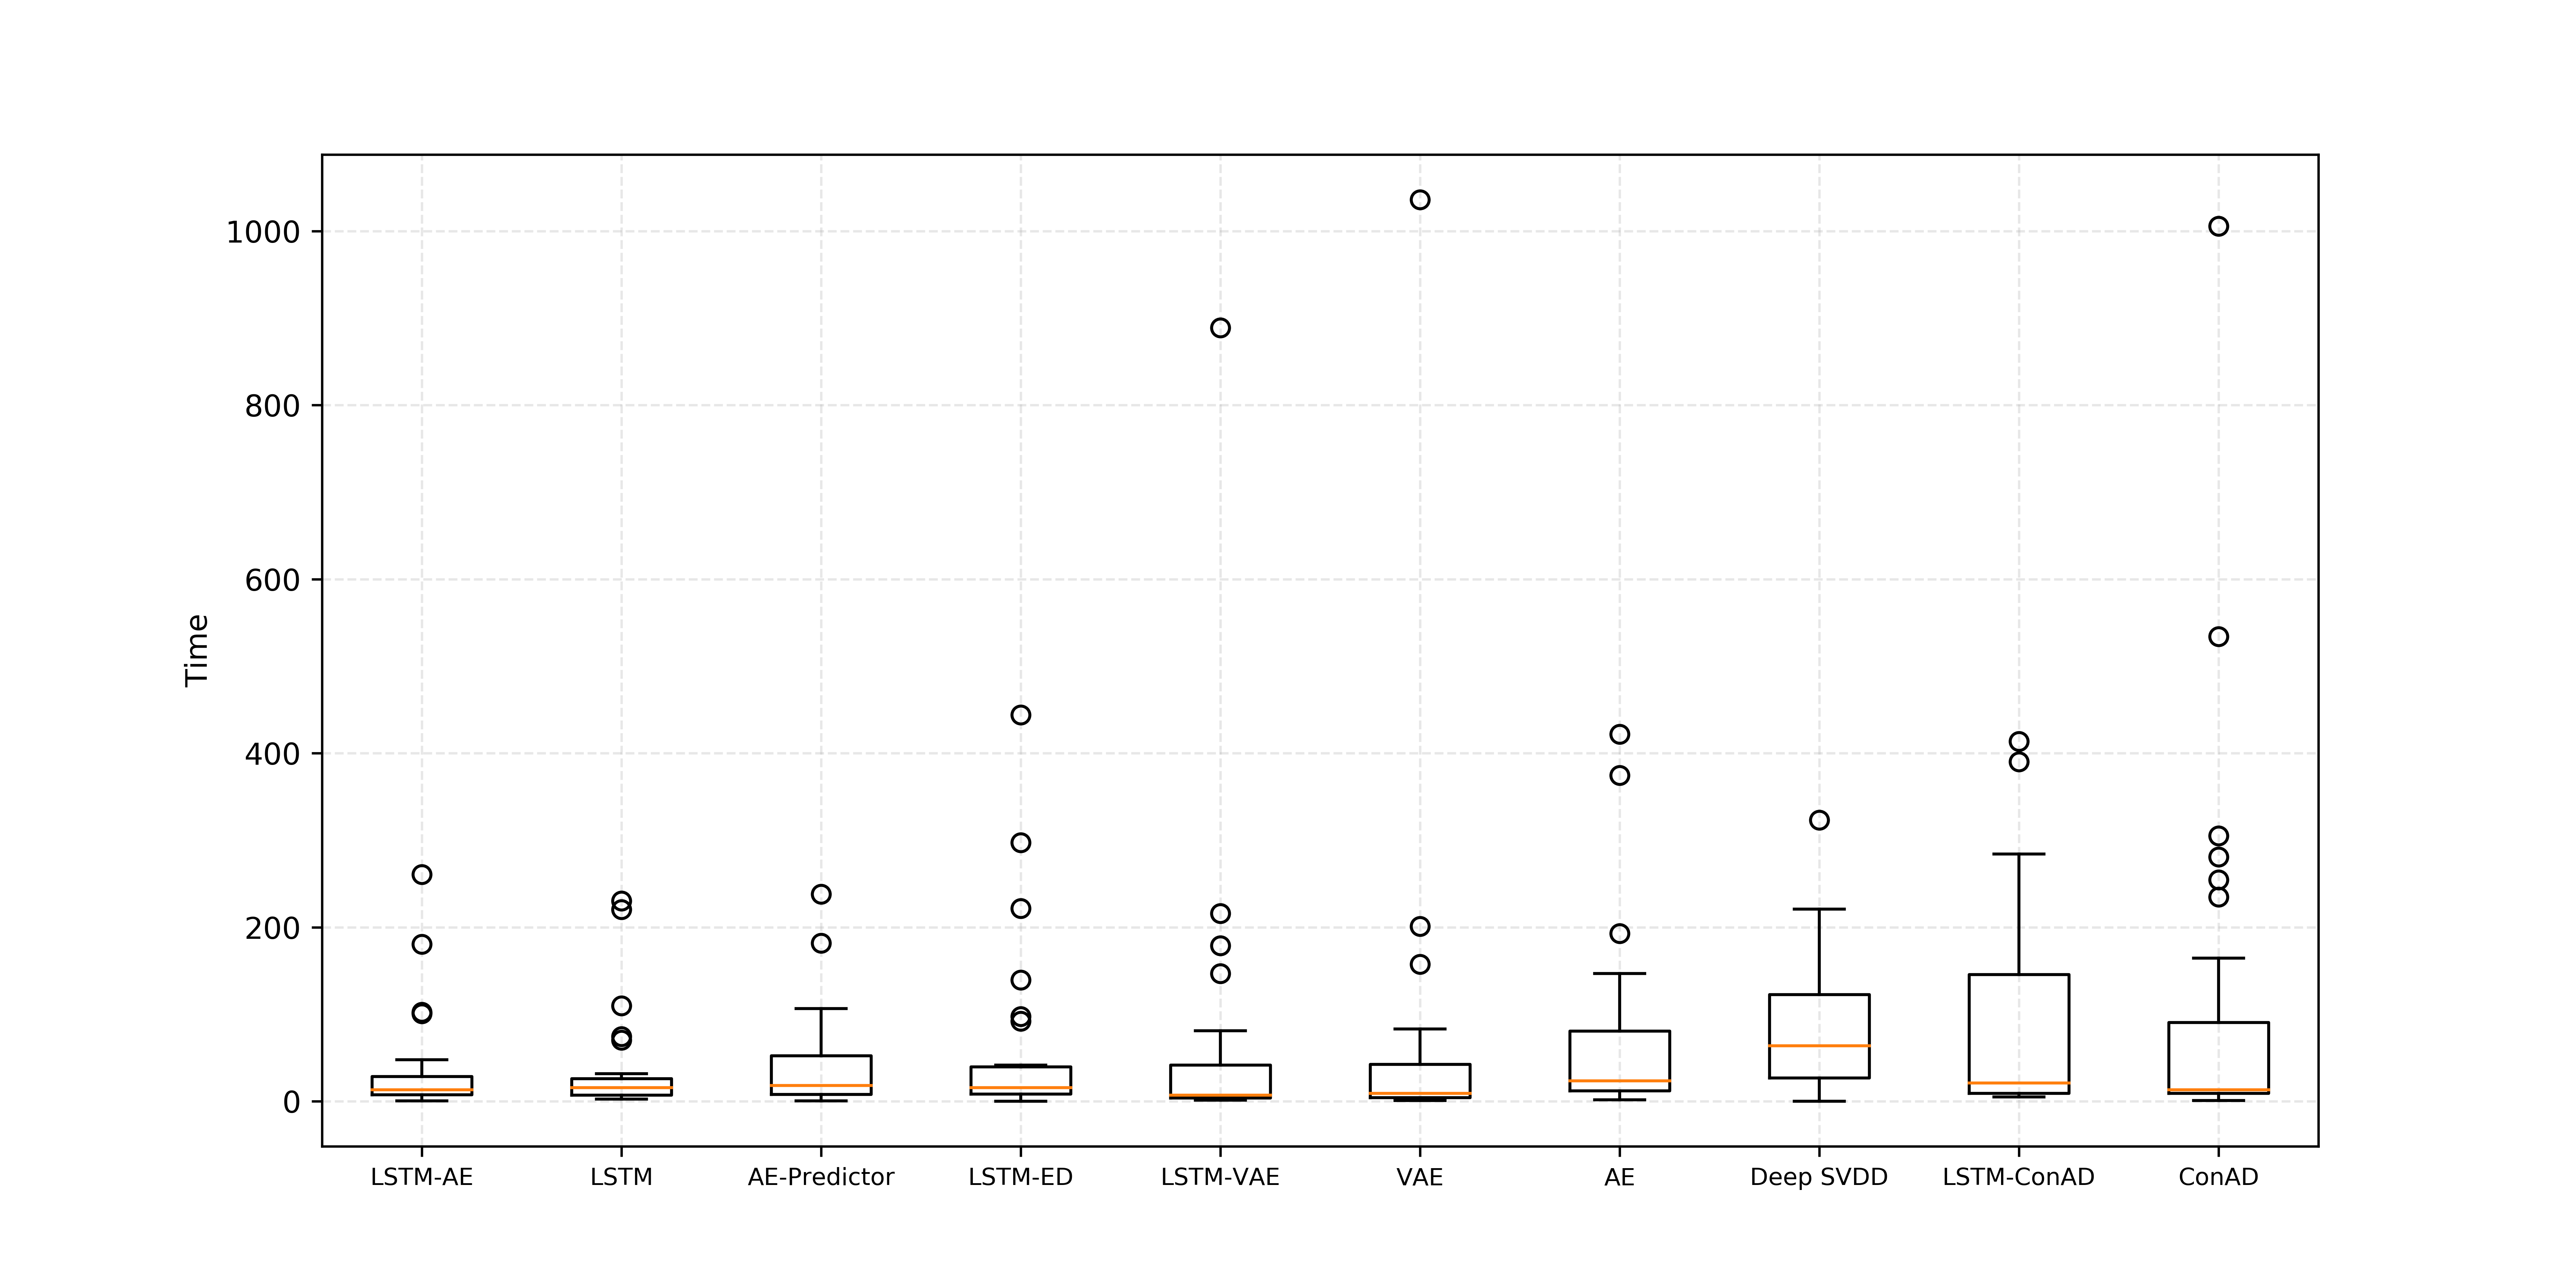
\includegraphics[width=\textwidth]{spot_time.png}
  \caption{POT方法评估时间}
  \label{fig:pot:time}
\end{figure}

图~\ref{fig:eval:time}则是所有算法用枚举所有阈值并选取最好的评估结果的耗时箱型图,从中看出用本文提出的方法进行评估的时间消耗较为稳定且快速,不依赖于算法的效果。

\begin{figure}[htbp]
  \centering
  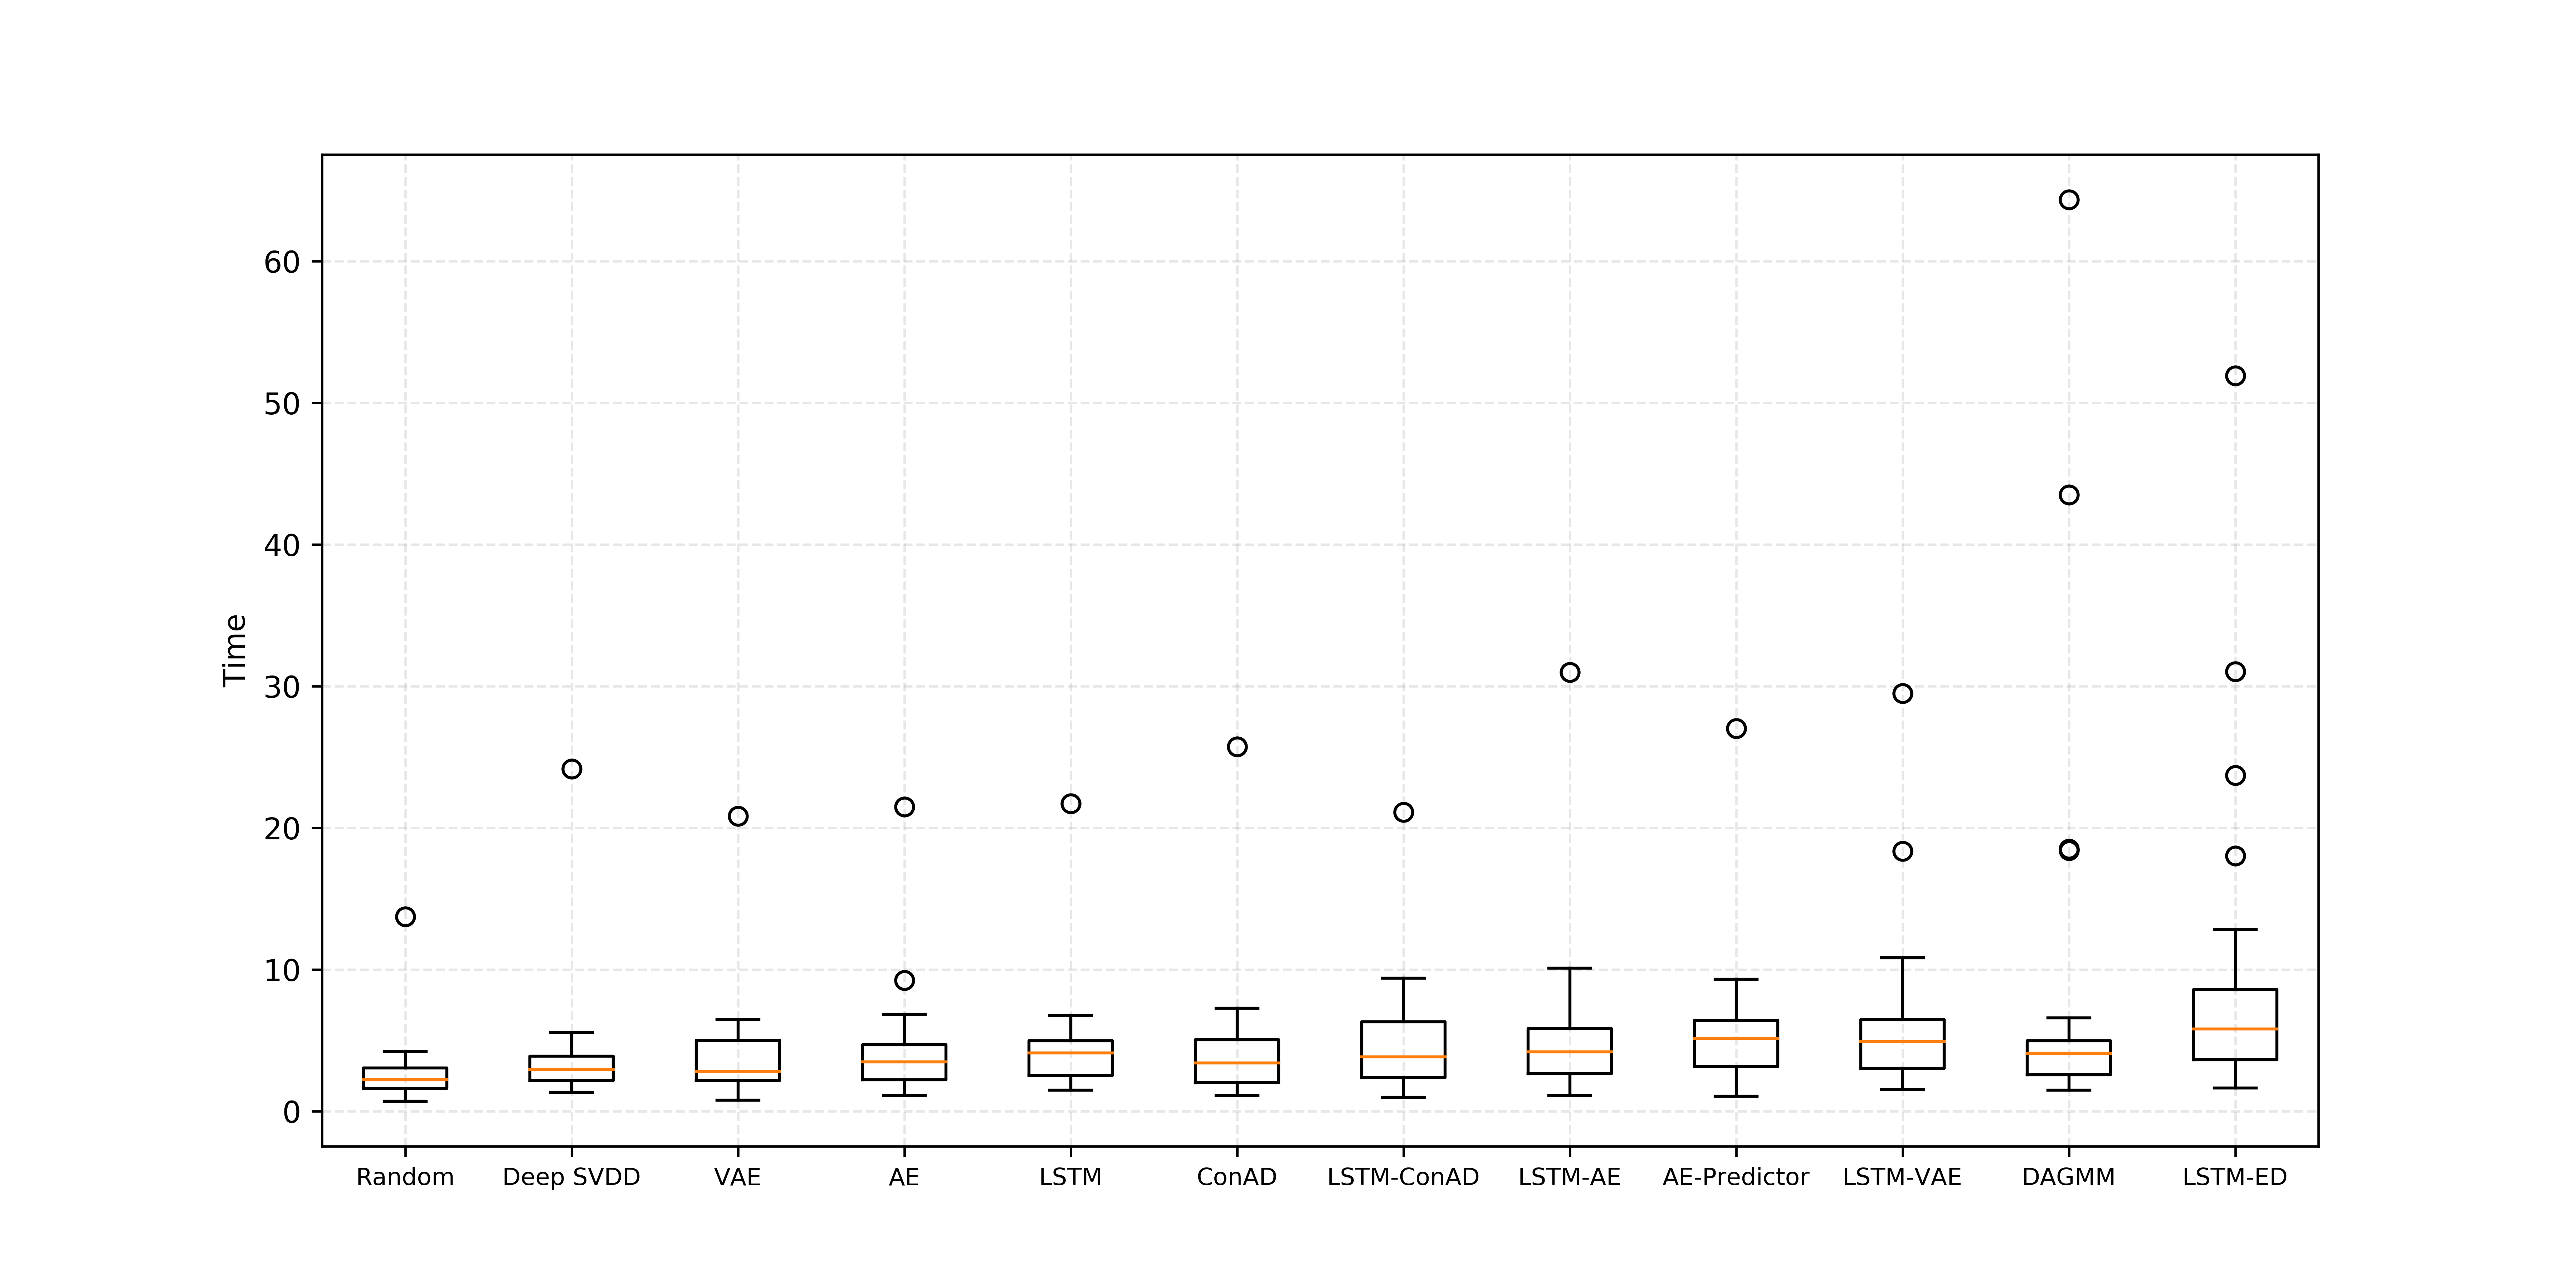
\includegraphics[width=\textwidth]{best_eval_time.png}
  \caption{枚举所有阈值评估时间}
  \label{fig:eval:time}
\end{figure}

\section{小结}
本章详细介绍了基于深度学习方法的时间序列异常检测框架各方面的设计思路,也对实现的算法在性能和效率上进行了综合的评估,将来如果有其他的算法也可以放到该框架内与其他算法进行比较。



% !TeX root = ../main.tex

\chapter{基于时间序列异常检测的根因分析系统设计与实现}
\label{cha:intro}
\section{问题描述}
在复杂系统中,无论是微服务还是云网络的场景,一方面,我们会得到单点的多个指标数据,也就是单个点上多条时间指标序列,而且由于可能是不同类型的点(例如微服务中的操作系统、数据库、容器、中间件以及云网络中的网关、交换机、虚拟机、物理机等),其指标的模式以及指标的个数都不相同。另一方面,复杂系统中当出现异常时异常会在系统中蔓延,在云网络中是通过服务调用的方式来传播,在云网络中则是流量收发包的方式。本文中我们认为这种点与点之间的拓扑是已知的。当在一个给定时间点发生一个大规模异常时,有可能有多个点以及多条链路发生故障,我们需要快速定位到是哪个节点最初发生故障并通过链路传播到了整个系统导致系统整体运行出现问题。

\section{框架设计}
本文设计的根因分析框架如图~\ref{fig:part2-overview}所示:
\begin{figure}[htbp]
    \centering
    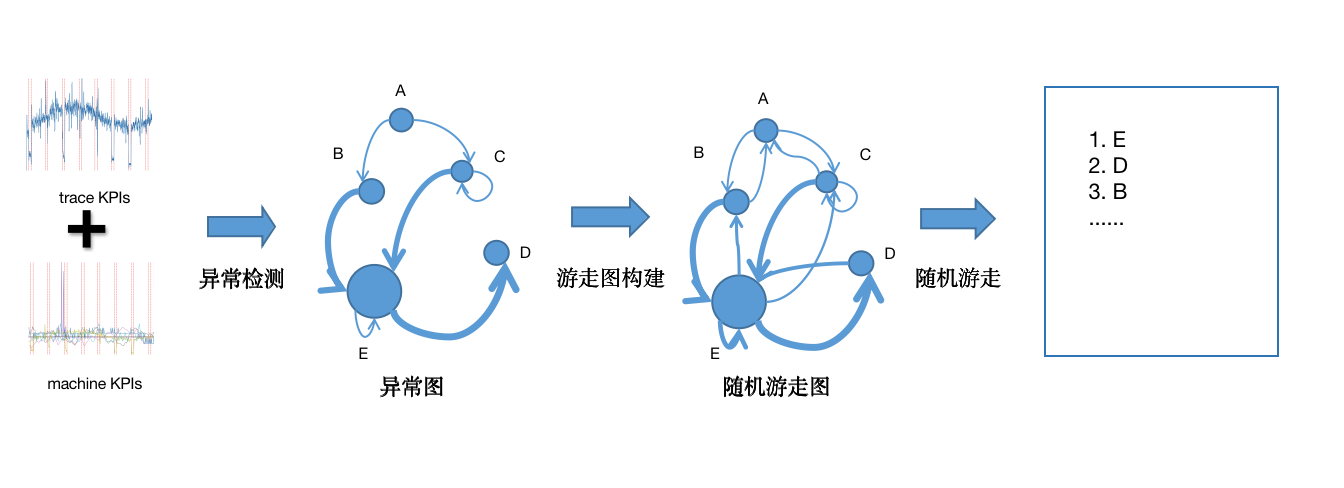
\includegraphics[width=\textwidth]{part2_overview.png}
    \caption{基于时间序列异常检测的根因分析系统框架}
    \label{fig:part2-overview}
  \end{figure}

首先通过预处理得到一系列节点上的时间序列数据和节点之间调用服务的相关指标(每分钟的调用次数、过去一分钟内的调用延时等)的时间序列数据,通过在故障时间点对这些时间序列数据运行异常检测算法得到这些曲线在该时刻的异常分数。用图的方式来可视化系统当前的状态:当一个节点的指标表现越异常,它的节点半径越大,如果一条边越异常,那么这条边就越粗。然后我们在这张图的基础上增加一些边以及修改一些边的权重,得到一张随机游走图。最后在图上运行随机游走算法来得到最有可能是根因的节点列表。接下来详细介绍各部分实现的细节。
\section{异常检测模块}
\label{sec:anomaly:detection}
在异常检测模块,需要在每个故障的时刻给出每个点以及每条边的异常程度。这部分当数据量足够大的时候可以直接使用第~\ref{cha:anomaly:detection}中使用的基于深度学习的方法,此处不再赘述;当数据量较小例如每个点只有几百个采样点的时候,可以对每个单条的时间序列数据运用基于统计的方法得到一个异常分数,然后再用某个聚合函数(例如最大值或者平均值)将多个时间序列数据的分数变成单点/边的异常分数。

具体来讲,当数据点较少时,本文选择了KDE\footnote{Kernel Density Estimation,核密度估计}算法来做异常检测,因为其计算简单、通用性强,适用于各种特性的时间序列数据,基本思路是查看故障时间点后一段时间数据的分布于前一段时间数据分布的拟合情况,两者差别越大认为该数据异常程度越高。但实际使用中发现这个做法存在两个缺陷:一是会被偶然的突刺影响到,而这种尖刺可能是统计错误或者其他原因造成的突发状况,但不足以构成异常;二是有明显长周期性的数据问题会影响到KDE算法的正确性,因为KDE只考虑了故障时间前后较短时间内的数据,因此如果有长周期特征的话,前后两个时间段的数据可能分布上来看有很大的差别但从长远上来看是符合历史特征的,这种不应该被判断为异常。因此本文选择在采用KDE算法之前去掉明显的突刺,以及减去周期性的数据,消除这两部分的影响。另一方面,因为要将多个时间序列数据的异常分数进行聚合,而不同的时间序列数据可能具有不同的量纲和数量级,直接用KDE的话本身数据偏高的数据计算得到的异常分数也偏高。所以为了将所有时间序列数据的异常分数放在一起比较的结果具有可靠性,我们需要先将所有数据做归一化。因此,异常检测这部分步骤总结如下:第一步做归一化,第二步去掉尖刺数据,第三步进行周期性检测,将周期性数据从原数据中减掉,最后一步再进行KDE异常检测,输出一个异常分数。
\subsection{归一化}
目前常用的数据归一化方法主要是min-max和z-score标准化,考虑到min-max受异常值影响较大,我们采用了z-score标准化的方法。设原始数据的值为$x_i$,$mean$为原始数据的平均值,$std$为原始数据的标准差,则:
\begin{equation*}
y_i = \frac{x_i-mean}{std}
\end{equation*}

$y_i$为归一化后的数据,均值为0,方差为1,而且没有量纲。
\subsection{去除尖刺}
去除尖刺的目的是为了消除统计错误,也就是数据中明显不符合正常数据的凸起,而且这种凸起往往是短时间内的,例如一个时间点的数据与前后两个相邻采集点的差距都过大,我们要去除这种情况。但我们不能采用将边缘的极值去掉的方法,因为我们想要检测的异常可能就是处于边缘的极值,但是这种异常和统计错误的区别就是持续时间会相对久一些(例如5分钟以上),因此本文针对做以下的平滑方式:
\begin{equation*}
z_i = \begin{cases} \frac{y_{i-1} + y_{i+1}}{2}, & y_i - y_{i-1} > th\ and\ y_i - y_{i+1} > th \cr \frac{y_{i-1} + y_{i+1}}{2} & y_{i-1} - y_i > th\ and\ y_{i+1} - y_i > th \cr y_i, & otherwise  \end{cases}
\end{equation*}

$z_i$则为去除尖刺后的数据。
图~\ref{fig:smooth}展示了一个去除突刺的示例。其中红色标红的是出现故障的区间,如果不去除这些尖刺可能会导致在计算KDE时将尖刺统计在内而出现问题,0:45左右是真正出现故障的时间,而其他时间的波动都是正常波动,而去除尖刺之后我们很好地保留了真正的故障时段的异常,而去除了其他时刻的尖刺,保证其他时刻不会被误报。

\begin{figure}[htbp]
  \centering
  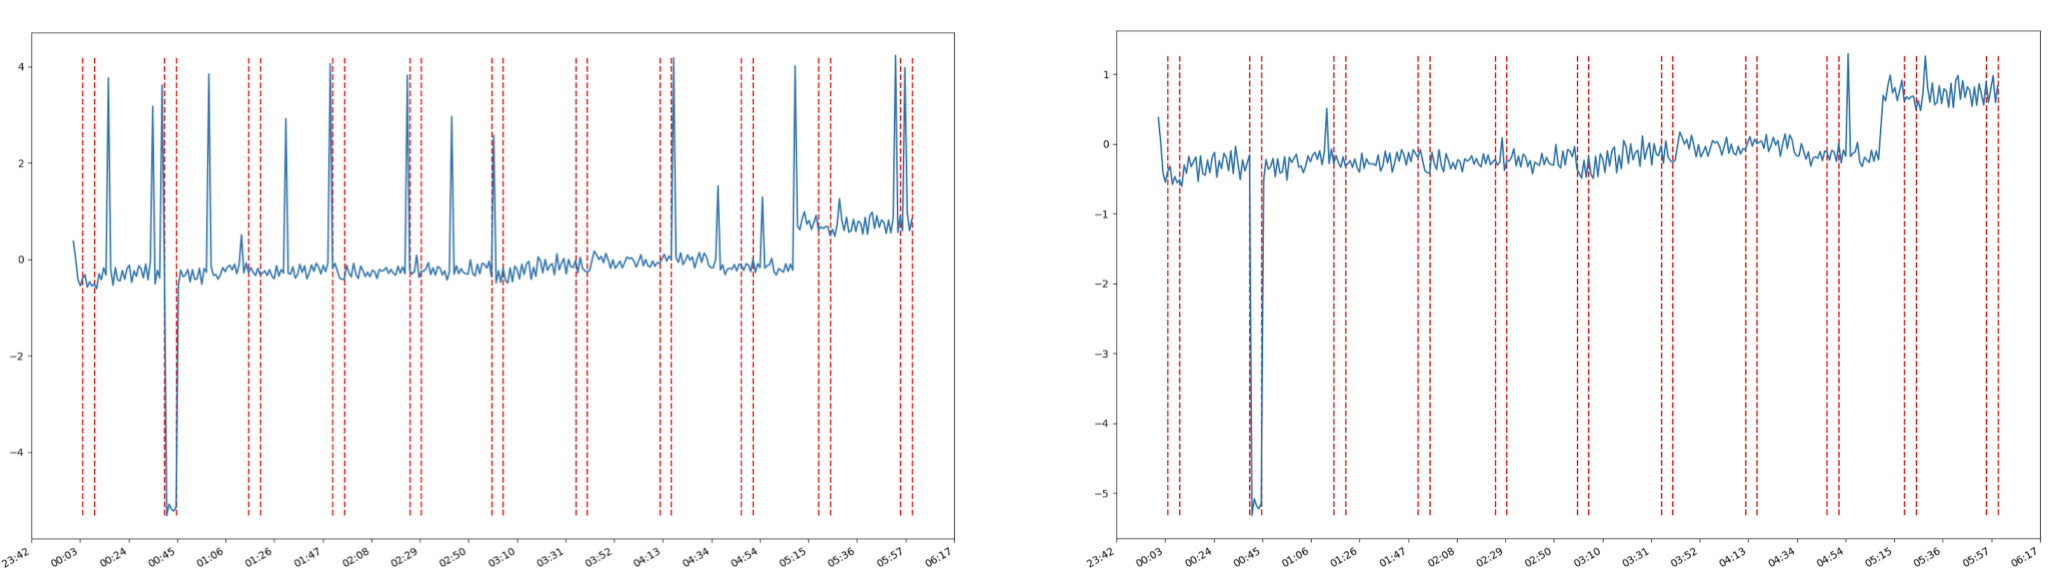
\includegraphics[width=\textwidth]{smooth.png}
  \caption{去除尖刺示例}
  \label{fig:smooth}
\end{figure}
\subsection{周期性数据去除}

在实际的时间序列数据中我们经常会遇到如~\ref{fig:period}左图所示的数据,具有很强的周期性,这样的数据完全是符合历史特征的,所以不应该被判断为异常。但如果我们用KDE算法的话,一个前提是当前数据只和周围数据相关,不会考虑到很久以前的数据,所以我们需要把周期性先给去掉。那么首先我们就要知道序列的周期是多长,这里我们用了自相关函数的方法,计算方法为:
\begin{equation*}
  acf_i = \sum_{j=1}^{N-i}z_j\times z_{j+i}
\end{equation*}

$acf$函数如图~\ref{fig:period}中间图所示,从画出的自相关函数图中找到第一个尖峰位置,就可以确立出函数的最小正周期为$T$(图例中最小正周期为120),然后再统计出周期内每个位置的平均数据,并且用原数据的每个位置减去他们在周期中所处位置平均值,相当于我们将原数据分解为两部分,周期性数据和残差数据。即:

\begin{equation*}
  \begin{aligned}
  m_i = \sum_{j\%T = i}z_j\\
  w_i = z_i - m_{i\%T}
  \end{aligned}
\end{equation*}

将周期性数据减去之后得到处理好的数据如图~\ref{fig:period:right}所示,可以看到处理前的曲线有大量的起伏,如果故障时间点在中间那么无一例外这些地方都会认为是异常,而处理之后的数据尽管还留有少部分的突刺(这是因为每两个尖峰之间的距离可能不能恰好的一个周期,因此在统计时没有完全对上),但大部分时间值的分布都在0附近,说明大部分时候该曲线还是符合历史特征,不会被报为异常。
\begin{figure}[htbp]
  \begin{subfigure}[b]{0.335\textwidth}
    \begin{minipage}[t]{\linewidth}
    \centering
    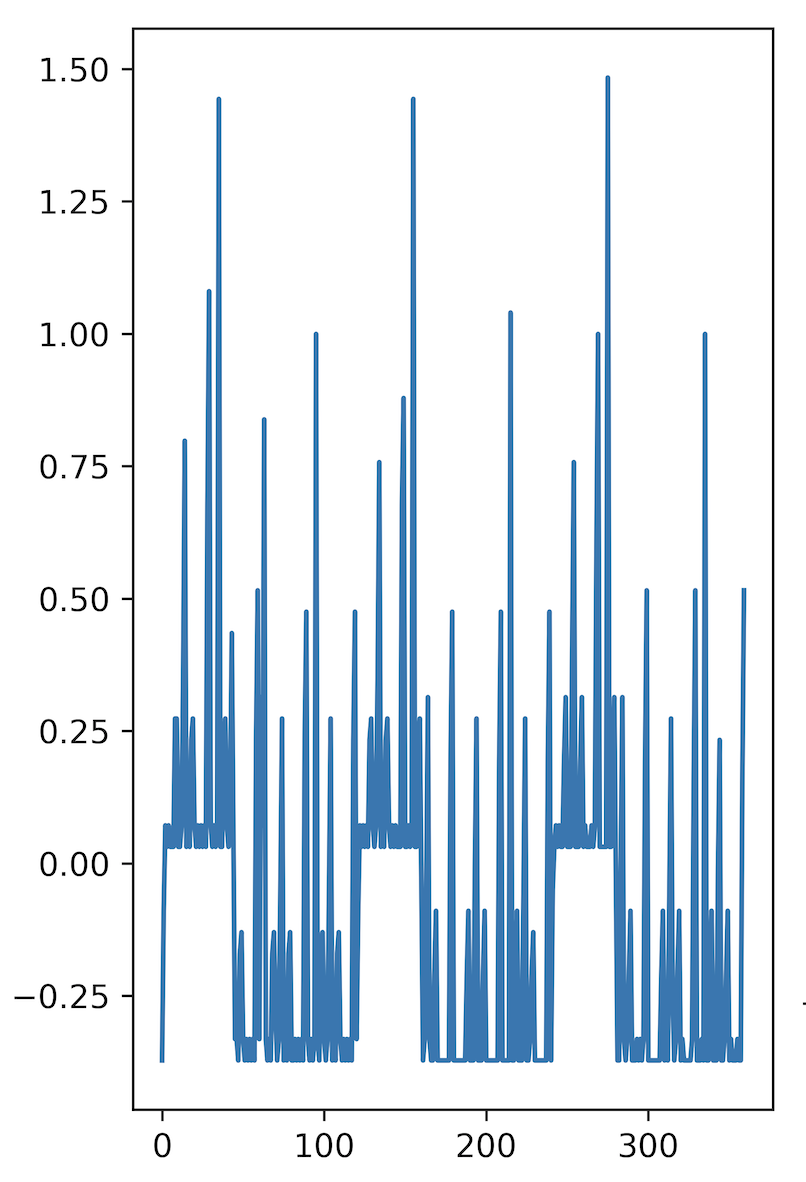
\includegraphics[width=\textwidth]{period_example_l.png}
    \caption{原始数据}
    \label{fig:period:left}
    \end{minipage}
  \end{subfigure}
  \begin{subfigure}[b]{0.325\textwidth}
    \begin{minipage}[t]{\linewidth}
    \centering
    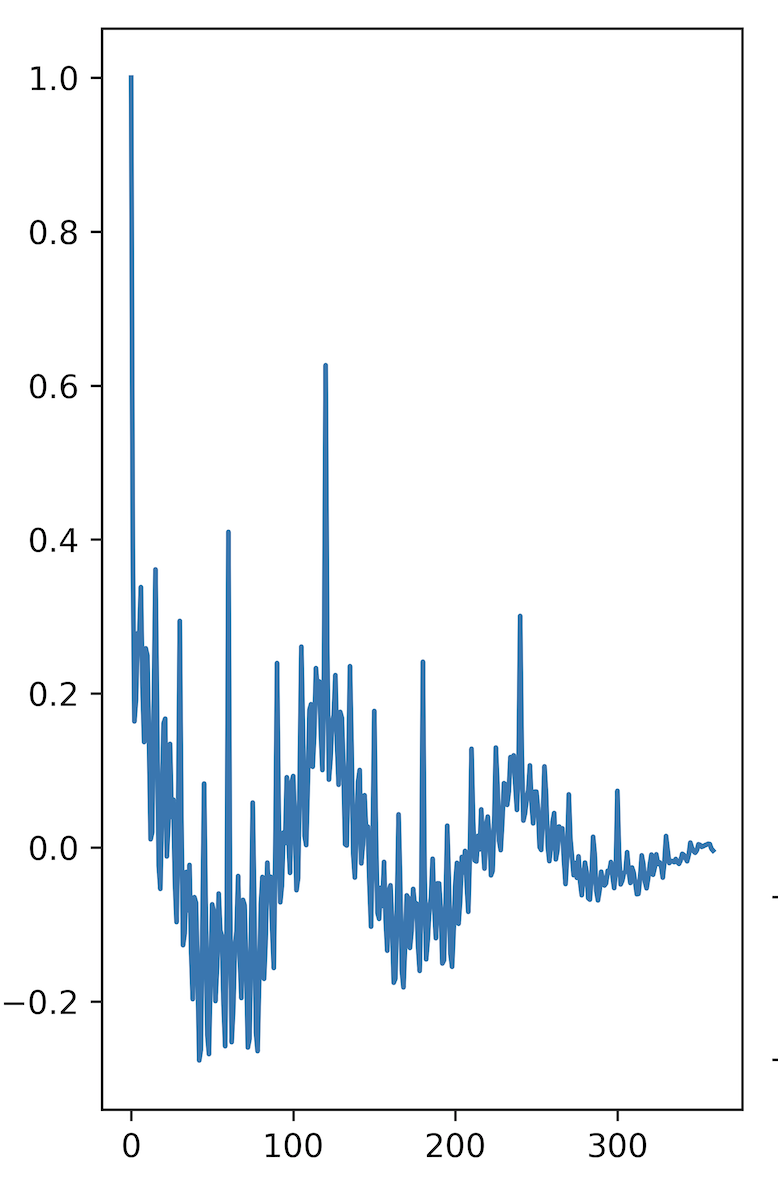
\includegraphics[width=\textwidth]{period_example_m.png}
    \caption{自相关函数}
    \label{fig:period:middle}
    \end{minipage}
  \end{subfigure}
  \begin{subfigure}[b]{0.325\textwidth}
    \begin{minipage}[t]{\linewidth}
      \centering
      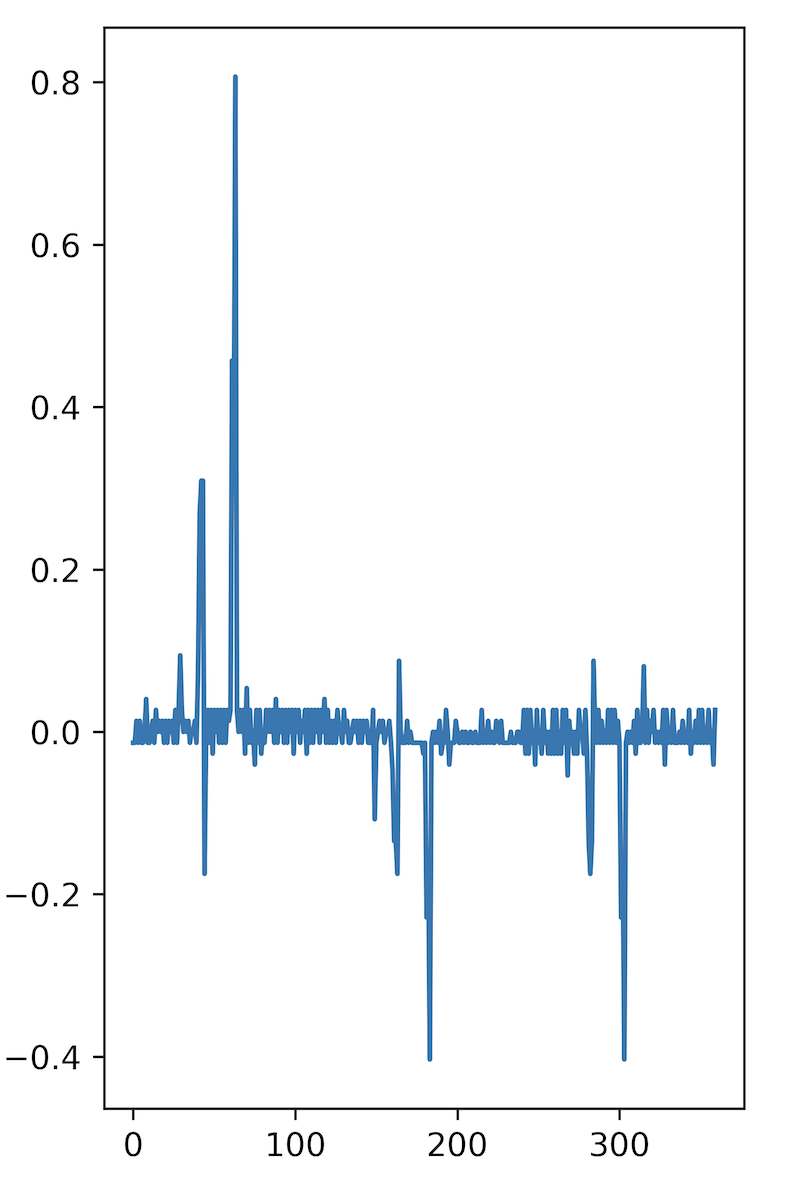
\includegraphics[width=\textwidth]{period_example_r.png}
      \caption{去除周期后的数据}
      \label{fig:period:right}
      \end{minipage}
    \end{subfigure}
    \caption{对数据去除周期化的过程}
    \label{fig:period}
\end{figure}
\subsection{KDE异常检测}
KDE是概率论中用来估计未知函数密度的非参数检验的方法之一,可以根据观察到的样本来估计随机变量的概率密度函数。本文将一条时间序列数据近似看为一个随机变量的多个采样值,然后用KDE来估计概率密度函数。
\begin{equation*}
\hat{P}(w) = \frac{1}{n}\sum_{i=1}^nK(w;w_i)
\end{equation*}

其中$K$是可选取的核函数,$n$则是采样个数。KDE的核心思想就是对每个采样点形成一个一定带宽的核函数然后将所有采样点的核函数叠加起来作为对该数据的分布估计,当有了密度函数之后,我们就可以用来计算新出现的数据概率了。当给出故障时间点时,我们用前$T_a$时间内的数据来估计出一个密度函数,然后再来评估故障发生之后$T_b$时间内数据出现的概率,概率越低说明这段时间的数据越异常,那么异常分数就越高。设之后$T_b$时间内的数据为$w_1,w_2,\dots,w_k$,而前$T_a$时间内的数据用KDE估计得到的密度函数为$\hat{P}(w)$,则异常分数为:
\begin{equation*}
  Score = \frac{1}{k}\sum_{i=1}^k\ln P(w_i)
\end{equation*}

其中求均值是为了消除$T_b$时间内不同曲线可能采样点个数不同带来的影响。

得到了每条时间序列数据在该时刻的异常分数之后,需要将多条曲线的值聚合到点或者边上。对于一个点来说,我们认为它的异常分数就是所有异常分数的最大值,因为这些时间序列数据之间可能是不相关的,比方说某个时刻内只有发包数发生了异常其他指标都工作正常,也足以认为是出现了异常;而对于边来说,因为有重边的存在,我们认为边的异常分数是所有重边的异常分数的平均值,因为这些数据是相关的,都是表示从一个节点调用另一个节点的服务情况,如果出现异常的话,所有的曲线应该都有一个较高的异常分数,如果只有一条曲线的分数较高则有可能是异常检测算法不准导致的偶然情况。至此我们得到了一张异常图,来描绘当前系统中各点和各边的异常情况,如图~\ref{fig:part2-overview}异常图所示。
\section{根因分析模块}
这部分要在异常图的基础上构建出随机游走图,再通过随机游走得出经过每个点的次数,经过次数越多则越可能是根因。


\subsection{构建随机游走图}
不妨设~\ref{sec:anomaly:detection}节得到的异常图为$G=(V,E)$,点$i$的点权为$v_i$,边权为$w_{i,j}$。要构建的随机游走图由以下三种边组成:
\begin{itemize}
  \item 前向边:为了运行随机游走算法,边的方向应当代表异常传播的方向。当一个$i$调用$j$的服务调用时长发生异常时,我们认为异常是由$j$传播到$i$,因此异常传播的方向与服务调用的方向相反,也就是根因的方向与服务调用的方向相同。所以该部分保持不变;
  \item 反向边:因为随机游走具有一定的随机性,为了防止行走者走到一个较小概率是根因的节点,然后出不去,我们考虑加入反向边。该边的权值随正向边的权值增加而增加,也就是$w_{i,j} = \rho_{back} w_{j,i}$,如果$(i,j) \notin E\ and\  (j,i) \in E$;
  \item 自环:当节点自身就是根因的时候,我们需要增大其留在原位置的概率而不走到其他地方。我们观察到:当一个节点是根因时,它会影响到周围和它有关联的点,通常情况下所有调用它的服务的返回时间的都会出现异常,同时它调用其他节点的服务也会出现异常,因此我们要将这些因素也纳入考量范围。总的来说我们需要考虑三个因素,一是节点本身的异常分数,二是所有其他节点到该节点的边的异常分数的平均值,三是该节点到所有其他节点的边的异常分数的平均值,也就是$w_{i,i} = \rho_{in} in\_avg\_weight_{i} + \rho_{out} out\_avg\_weight_{j}+ \rho_{self}  v_i$。另一方面,考虑到入边是推导根因的方向,所以我们在设置超参时会保证$\rho_{in}>\rho_{out}$。
\end{itemize}

总结如下:
\begin{equation*}
w_{i,j} = \begin{cases} w_{i,j}, & if\ (i,j) \in E \cr \rho_{back} w_{j,i}, &\ if\ (i,j) \notin E\ and\  (j,i) \in E \cr \rho_{in} in\_avg\_weight_{i} + \rho_{out} out\_avg\_weight_{j}+ \rho_{self}  v_i, & if\ i=j \end{cases}
\end{equation*}

\subsection{随机游走}
首先将边权矩阵$w$标准化得到转移矩阵$\overline{w}$:
\begin{equation*}
  \overline{w}_{i,j} = \frac{w_{i,j}}{\sum_jw_{i,j}}
\end{equation*}

然后在整张图中随机起点开始行走,当处于位置$i$时,有$p$的概率随机到达图中任一位置,有$1-p$的概率沿图中的边行走,而到达相邻点$j$的概率就为$(1-p)\overline{w}_{i,j}$,行走一定的次数之后,统计每个点被经过的次数,经过次数越多的则越有可能是根因。随机游走过程如算法~\ref{algorithm:random:walk}所示。

\begin{algorithm}
  \caption{随机游走过程}
  \begin{algorithmic}[1]
      \Require $p,V,\overline{w},step$
      \Ensure $R$
      \State $v$ \gets randomly choose from $V$
      \Repeat
      \State $r \gets random(0,1)$
      \If {$r < p$}
        \State $v$ \gets randomly choose from $V$
      \Else
        \State $v$ \gets randomly choose $j$ by $\overline{w}_{v,j}$ probability
      \EndIf
      \State $R_i \gets R_i + 1 $
      \Until {$step$ rounds}
      \State sort $R$ in descending order
  \end{algorithmic}
  \label{algorithm:random:walk}
\end{algorithm}
\section{实验评估}
本文采用AIOPS2020挑战赛作为验证算法效果的数据集。

\subsection{数据集介绍}

该数据集是一个微服务场景下的复杂系统数据集,整个系统如图~\ref{fig:static_topo}所示。提供了所有节点包括操作系统、容器和数据库的指标以一定时间间隔采样得到的指标信息,并且还有不同节点之间调用服务的记录。实际测试中,我们会得到若干个时间段,表示在这个时间段上整个系统出现了问题。需要我们找出的根因分为网络故障和节点故障,节点故障需要我们给出某个节点的某个指标,而网络故障如果在主机上需要给出指标,否则只需要定位到节点即可。具体的故障信息如表~\ref{tab:error}所示。

\begin{figure}[htbp]
    \centering
    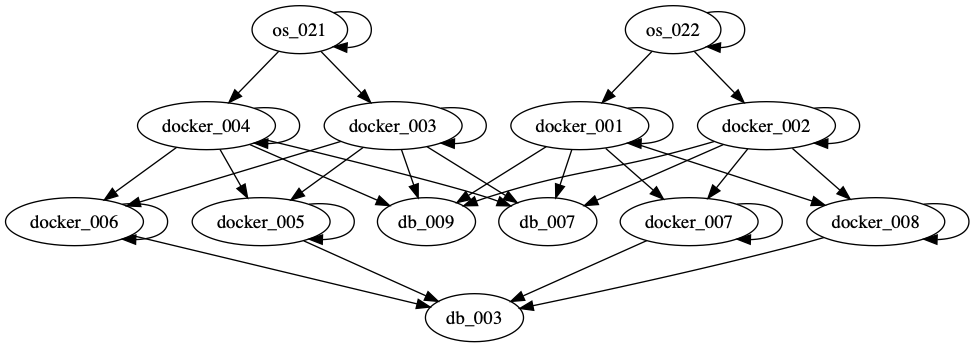
\includegraphics[width=\textwidth]{static_topo.png}
    \caption{静态拓扑图}
    \label{fig:static_topo}
  \end{figure}

\begin{table}
  \centering
  \begin{tabular}{ccc}
    \toprule
    技术栈 & 场景名称 & 定位需求\\
    \midrule
    \multirow{2}{*}{数据库oracle} & 数据库关监听 & 节点指标\\
     & 数据库连接限制 & 节点指标 \\
    \multirow{3}{*}{DCOS容器} & CPU压测 & 节点指标\\
     & 网卡丢包 & 节点\\
     & 网卡延迟 & 节点\\
    \multirow{2}{*}{主机} & 网络丢包& 节点指标\\
    & 网络延迟 & 节点指标\\
    \bottomrule
  \end{tabular}
  \caption{根因类别}
  \label{tab:error}
\end{table}

\subsection{实验设置}
超参数的设置方面,KDE算法中本文采用了高斯核函数,带宽取0.4,选择故障前后时间窗口的部分因为该数据集的故障持续时间均为5分钟,故$T_a$设置为15分钟,$T_b$设置为5分钟;根因定位方面构图的超参根据经验依次设置$\rho_{back}=0.5, \rho_{in} = 0.6, \rho_{out} = 0.3, \rho_{self} = 0.5$,随机游走的$p$设置为$0.1$,$step$则设置为10000步。

在结果输出方面,有两个要特别注意的地方。一是在该数据集中,存在两个容器例如docker001和docker005位于同一个主机os017上而该主机不出现在拓扑图上的情况,如图~\ref{fig:two:rca}所示,docker001和docker005像两个独立的根因,这种情况下要定位到os017。本文的做法是选取随机游走经过次数前二的点,判断其是否均为容器且位于同一主机上,如果是则定位到它们所属的主机上;另一个则是该数据集要求定位到具体的指标,如果是网络异常则不用输出指标。通过观察发现,网络异常往往的表现就是本身指标没有过于异常的,所以本位在定位到节点之后找到异常分数最大的指标,如果其指标异常分数大于某个阈值认为它是根因,否则认为是网络故障。

\begin{figure}[htbp]
  \centering
  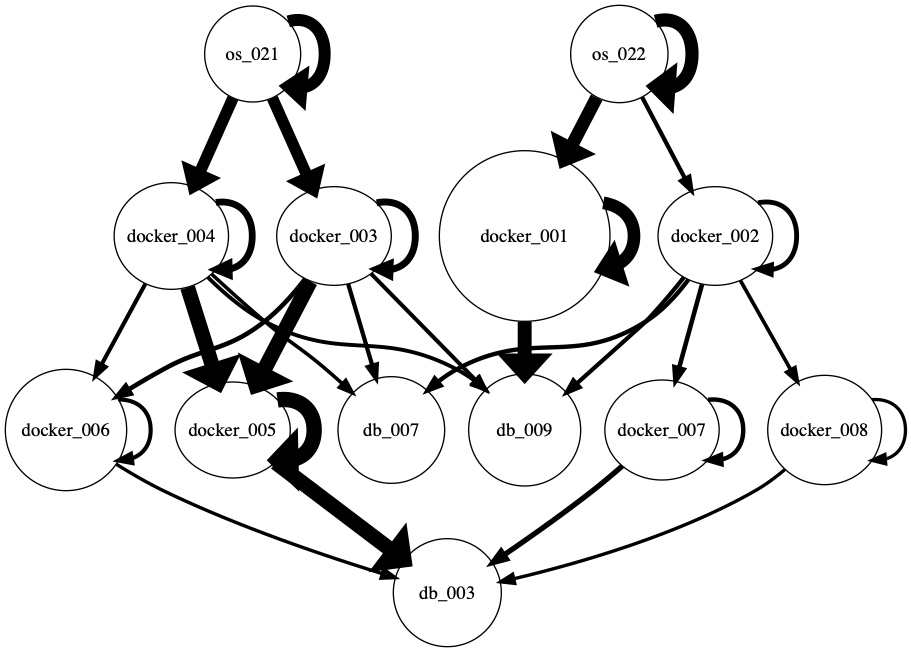
\includegraphics[width=\textwidth]{two_rca.png}
  \caption{数据集中的一个特例}
  \label{fig:static_topo}
\end{figure}


\subsection{baseline选取}
本文选取的baseline为在异常检测之后根据自身的异常分数以及相连边的异常分数之和排序然后选取最高的作为根因,在结果输出时与我们的方法保持一致。
\subsection{实验结果分析}
该数据集一共有5批数据,分别有11、11、3、10和10个测试点,本文的方法与baseline的方法在各批数据的正确率如表~\ref{tab:rca:result}所示。

\begin{table}
  \centering
  \begin{tabular}{ccccccc}
    \toprule
      & 第一批 & 第二批 & 第三批 & 第四批 & 第五批 & 总体\\
    \midrule
    baseline &  0.91 & 0.91 & 1 & 0.9 & 0.91 & 0.91\\
    ours & 0.64 & 0.73 & 1& 0.6 & 0.91 & 0.76\\
    \bottomrule
  \end{tabular}
  \caption{根因定位准确率对比}
  \label{tab:rca:result}
\end{table}

从中可以看出,使用随机游走的方法比直接在异常图上进行统计的方法准确率高出十五个百分点。而我们的方法未能准确检测的三个根因中有两个是根因和所得到的静态拓扑图完全没有关系的,而另两个则如图~\ref{fig:bad:case}所示。真正的根因是docker001的网络故障,而我们的算法定位到了os022的网络故障上,docker001在经过次数中排名第三位。所以在这种影响范围较小的情况下我们的算法准确性会出一点问题。而一些准确定位的故障其异常图如~\ref{fig:error:example}所示。当出现容器网络这一类故障例如图~\ref{fig:error:docker:network}时,baseline的方法则有可能会定位到os022,而随机游走则会避免这一错误,通过在图上不断地游走,最后经过正确答案也就是docker007的次数最多,并且,当系统的规模扩大时,baseline针对单点的统计更有可能出错,因为当调用链的长度增加时,会出现多个节点的异常分数与边的异常分数之和极大的情况,而真正的根因则需要用随机游走的方式,通过模拟异常传播的方式才能从调用链上推断出来。
\begin{figure}[htbp]
  \centering
  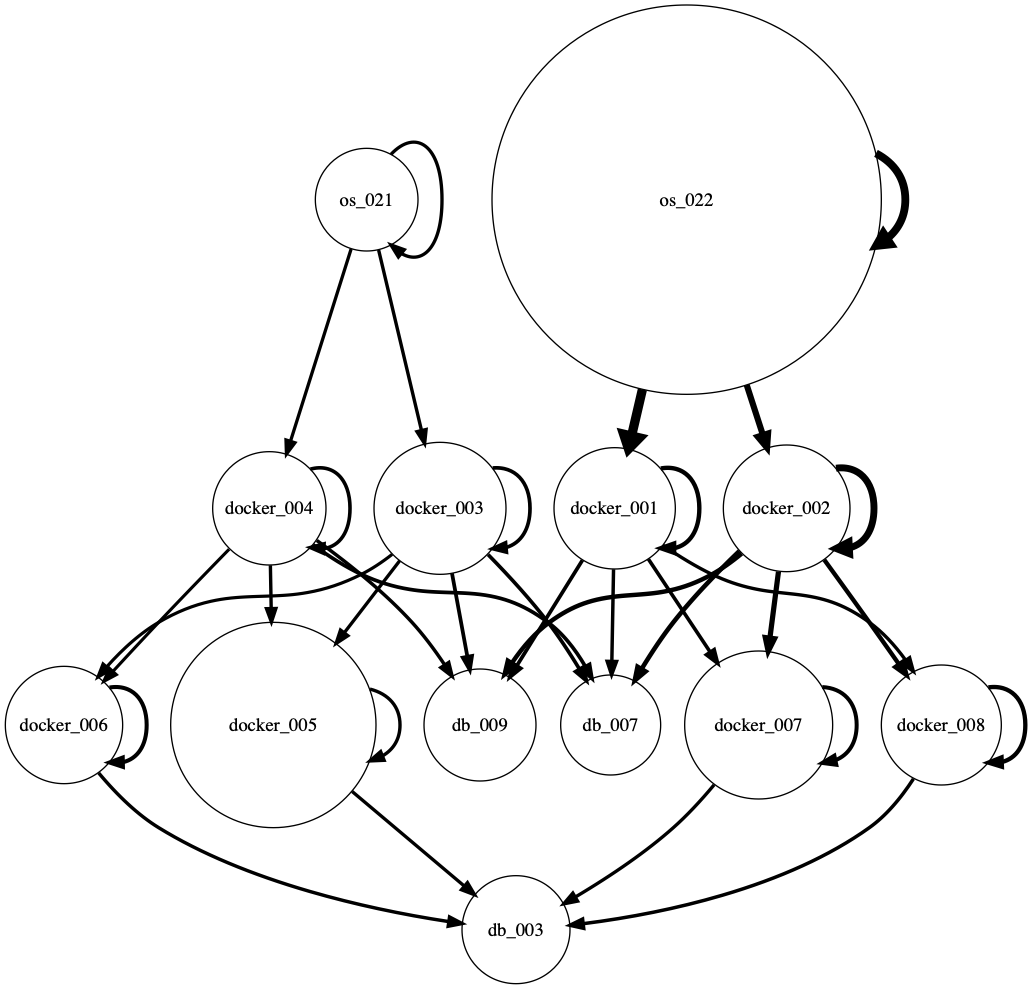
\includegraphics[width=\textwidth]{bad_case.png}
  \caption{本文算法的一个bad case}
  \label{fig:bad:case}
\end{figure}

\begin{figure}[htbp]
  \centering
  \begin{subfigure}[b]{\textwidth}
    \begin{minipage}[t]{0.5\linewidth}
      \centering
      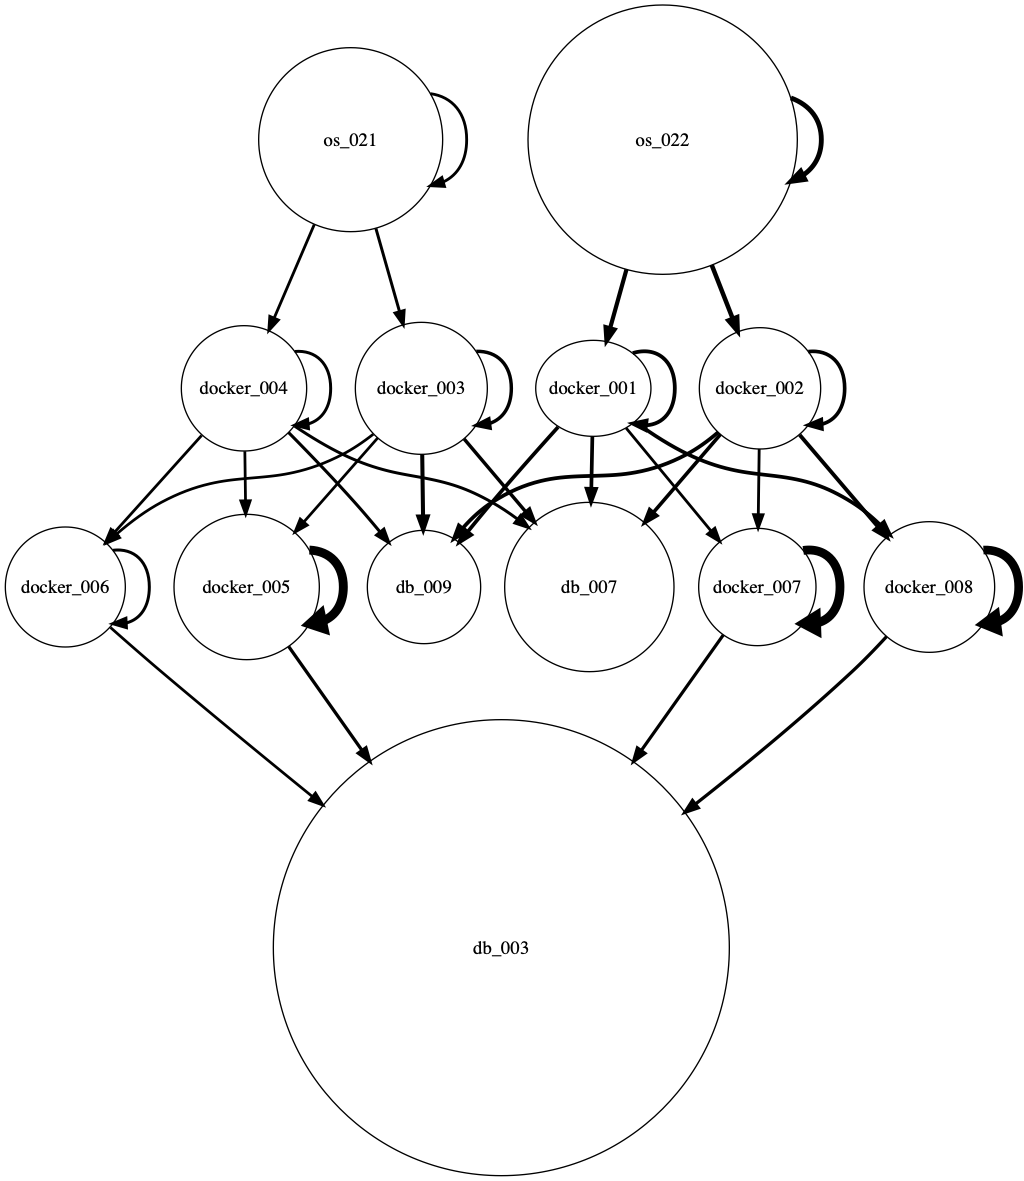
\includegraphics[width=\textwidth]{db_error.png}
      \caption{数据库关监听}
      \label{fig:error:db}
    \end{minipage}
    \begin{minipage}[t]{0.5\linewidth}
      \centering
      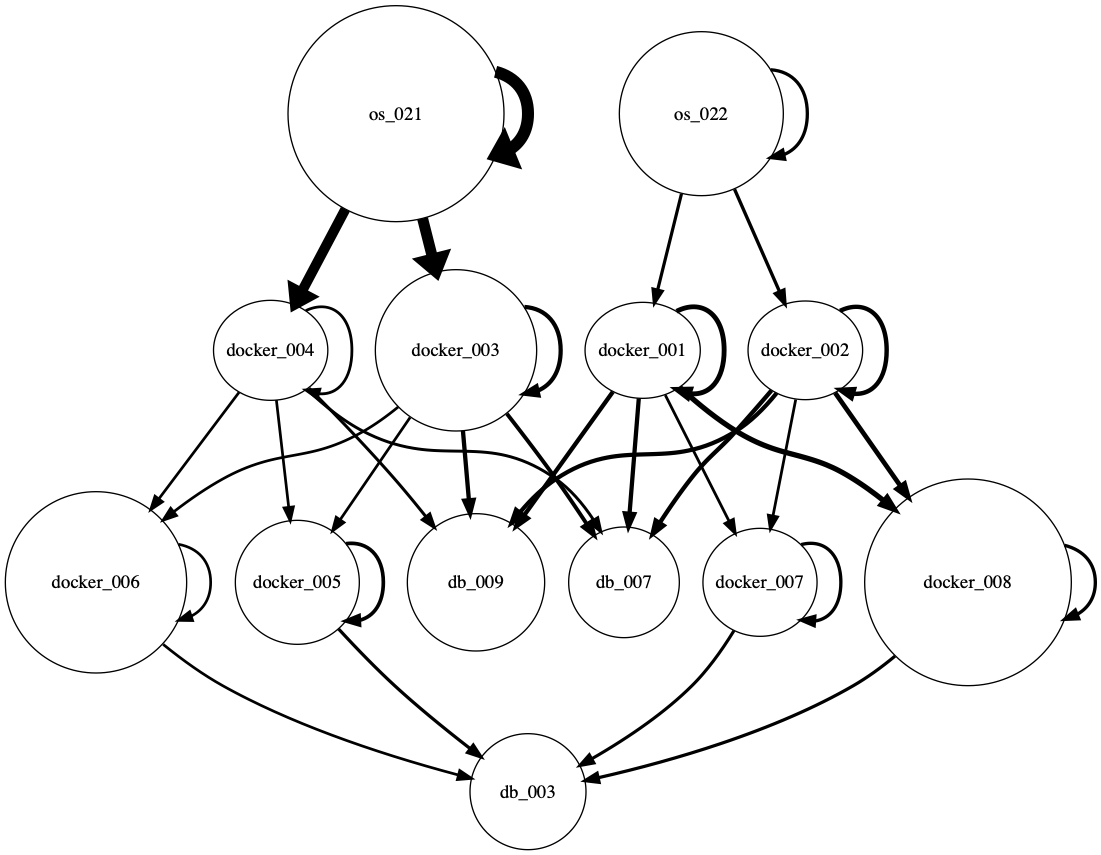
\includegraphics[width=\textwidth]{os_error.png}
      \caption{主机网络故障}
      \label{fig:error:os}
    \end{minipage}
  \end{subfigure}

  \begin{subfigure}[b]{\textwidth}
    \begin{minipage}[t]{0.5\linewidth}
      \centering
      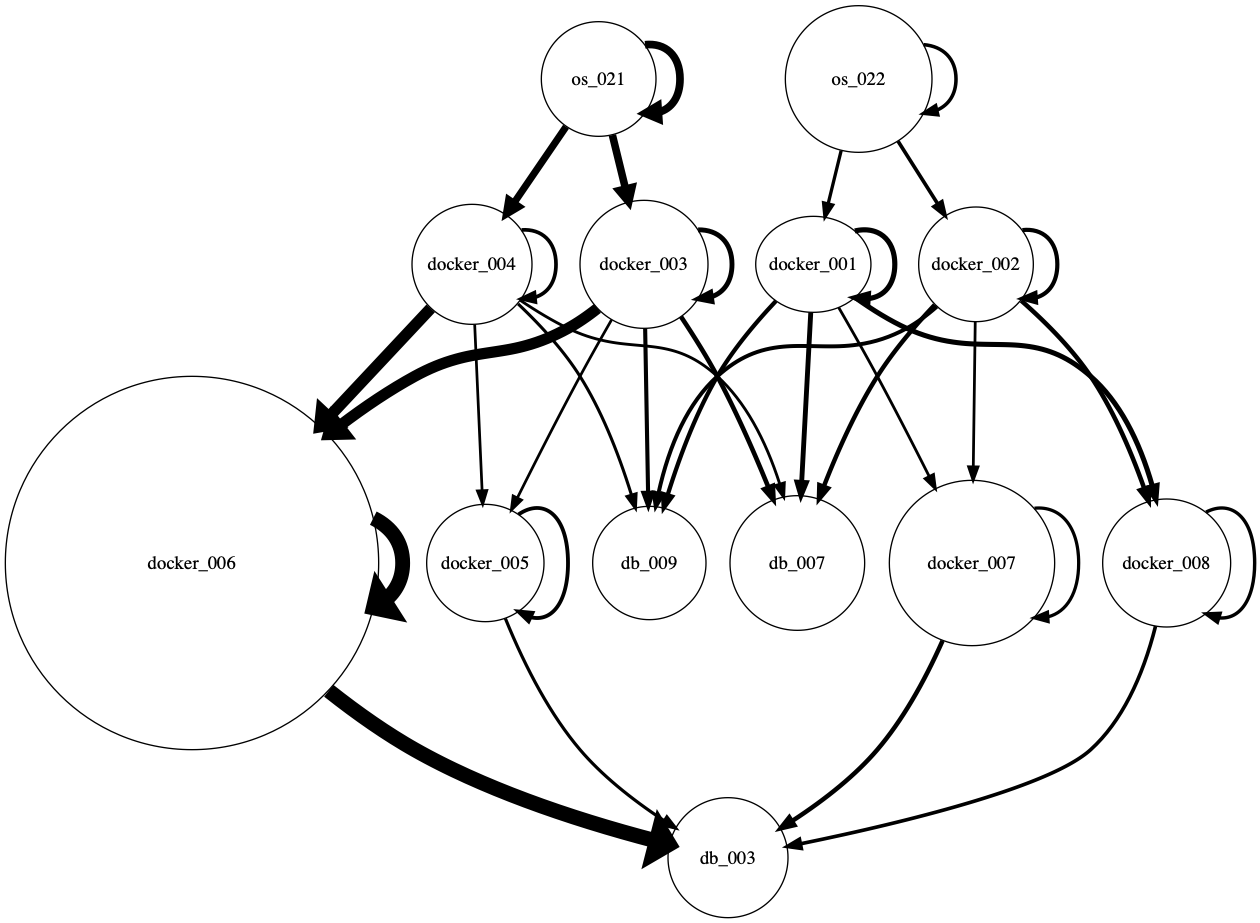
\includegraphics[width=\textwidth]{docker_cpu_error.png}
      \caption{容器cpu压测}
      \label{fig:error:docker}
    \end{minipage}
    \begin{minipage}[t]{0.5\linewidth}
      \centering
      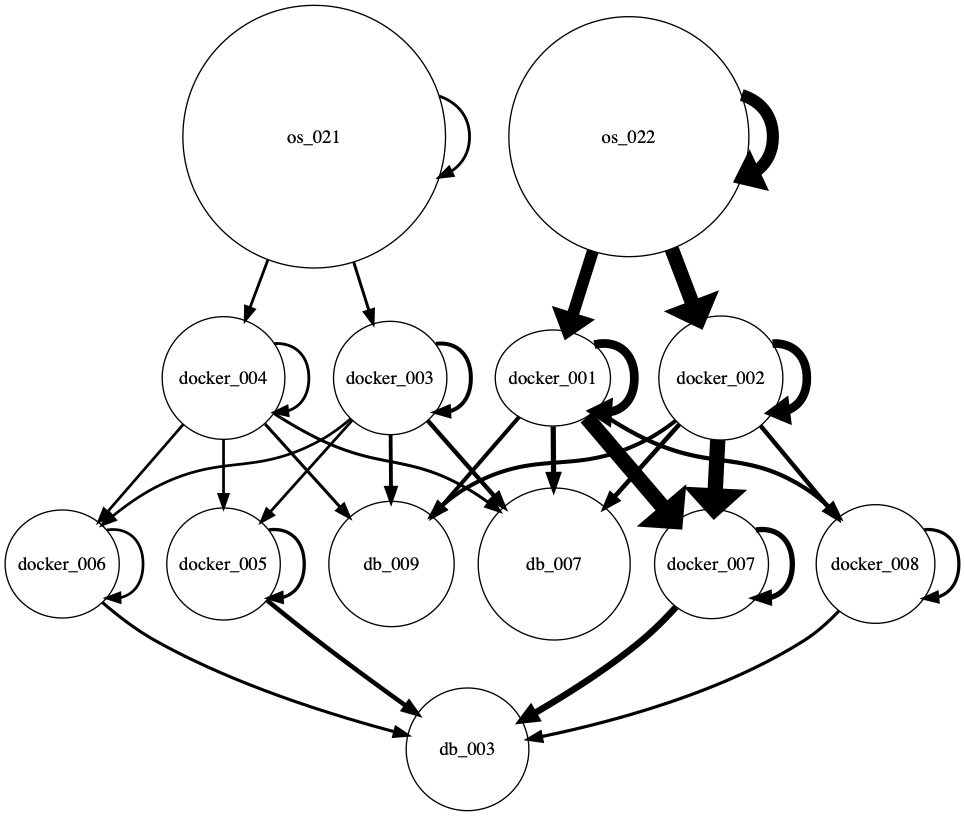
\includegraphics[width=\textwidth]{docker_network_error.png}
      \caption{容器网络故障}
      \label{fig:error:docker:network}
    \end{minipage}
  \end{subfigure}
  \caption{AIOPS2020挑战赛中故障示例}
  \label{fig:error:example}
\end{figure}

\section{小结}
本章详细介绍了基于时间序列异常检测的根因分析系统,对节点上的时间序列数据和节点之间的服务调用相关的时间序列数据运行KDE异常检测算法得到异常分数,以此为基础构建异常传播图,在这个图上进行随机游走算法来得到每个节点的经过次数,最多的即认为是根因。所用方法在AIOPS2020上验证得到了较高的准确率。
% !TeX root = ../main.tex

\chapter{总结与展望}
\label{cha:intro}
本文实现了基于深度学习的时间序列异常检测框架和基于时间序列异常检测的根因分析系统两个部分的工作,前者主要是在一个合理的评价标准以及统一的数据集上实现了已有的多种算法,也对已有的单点异常检测算法与时序模型结合提出了一些新的模型,在效果上有小幅的提升,但随之带来的是耗时的大幅增长,总体来讲并不划算,但该框架可用于之后与其他算法的横向比较;后者主要不同于以往的工作以时间序列数据的相关性为边权,我们提取出和边有关的时间序列数据(例如调用次数、返回耗时等),将时间序列异常检测的结果作为边权,结合点上的时间序列异常检测提供的点权,在有网络拓扑的前提下构建出了异常传播图,在图上运行随机游走算法来找根因,在AIOPS2020挑战赛中进行验证,得到了0.91的准确率。

同时,本文还有很多值得深入研究的地方。未来进一步的研究工作为:
\begin{enumerate}
    \item 没有将前后两者的工作形成一个完整的整体。前者的时间序列异常检测模型应该服务于后者的根因分析系统,但在评测时由于数据量的问题我们在根因分析系统中没能采用基于深度学习的方法;
    \item 时间序列异常检测的框架只采用了SMD一个数据集,虽然是出于其与云网络的场景较为相似而使用,但算法的效果不应该依赖于数据集的类型,只用一个数据集得出的结果很有可能有偶然性,可以增加数据集的使用,研究算法在不同数据集下的通用性;
    \item POT的方法在实验中发现对超参的选取十分敏感,同时耗时也不稳定,所以在落地上仍然具有一定的困难,还需继续探索其他自动确立阈值的方法;
    \item 将设计的系统实际部署到云网络中进行使用,还要考虑数据量的问题、通用性、检测效率等等问题是否满足要求。
\end{enumerate}




% 其它部分
\backmatter

%% 本科生要求的几个索引。
\listoffigures    % 插图索引
\listoftables     % 表格索引
%\listofequations  % 公式索引

% 参考文献
% \bibliographystyle{thuthesis-numeric}      % 顺序编码制
% \bibliographystyle{thuthesis-author-year}  % 著者-出版年制
\bibliographystyle{thuthesis-bachelor}     % 本科生参考文献的著录格式
\bibliography{ref/refs}s

% 致谢
% !TeX root = ../main.tex

\begin{acknowledgements}

\end{acknowledgements}


% 声明
\statement

% 附录
\appendix
% !TeX root = ../main.tex

\begin{survey}
\label{cha:survey}

\title{Research report}
\maketitle

My investigation is mainly divided into three progressive parts, the first part is a single time series data anomaly detection algorithm, the second part is a multi-dimensional time series data anomaly detection algorithm, and the last part is the root cause analysis of multi-point anomalies. Due to the particularity of the anomaly detection problem: it is difficult to define anomalies and it is difficult to obtain labeled data, so most of the survey methods are conducted in an unsupervised, zero-positive background.

Single time series data anomaly detection algorithm: \cite{malhotra2015long} is the first time to apply long short term memory networks to time series data anomaly detection. Previous work was performed in sliding windows, and the information obtained was limited, and the emergence of LSTM solved long-range dependence in this problem. \cite{DBLP:conf/kdd/RenXWYHKXYTZ19} linked the saliency detection of the visual direction with the abnormal detection of the time series data, thinking that the anomalies of the time series data also have similar saliency, so borrowed the most advanced models in saliency detection which are unsupervised spectral residual and supervised convolutional neural network. They use the output of the former as the input of the latter to form an SR-CNN model, which has achieved great performance and implemented a complete online / real-time time series data anomaly detection platform.

Multi-dimensional time series data anomaly detection algorithm: \cite{DBLP:journals/tdsc/WatsonSMMH16} use one class support vector machine to perform manual anomaly detection on system-level and network-level features, which ensured high efficiency while responding to anomalies never seen before. In \cite{DBLP:conf/ndss/MirskyDES18} a method using multi-layer AutoEncoder for feature reconstruction named Kitsune is proposed to perform multi-dimensional time series correlation data anomaly detection for network intrusion detection, in which a large number of original features and two-dimensional features are extracted, and the the feature incremental calculation method has greatly improved the efficiency of the algorithm so that it can support online intrusion detection. In \cite{DBLP:conf/aaai/ZhangSCFLCNZCC19}, a multi-dimensional time series correlation matrix is constructed to transform it into a two-dimensional matrix input, and then a complex fully convolutional networks is used to perform two-dimensional reconstruction. Although the model is more complex, the effect is relatively intuitive and interpretable. First, we can easily determine whether anomalies have occurred by determining the reconstruction loss threshold, and the root cause of the anomalies can be located by observing the distribution of the loss. However, this method of forcibly converting one-dimensional data to two-dimensional data may be inadequate. It also does not have spatially very strong spatially dependent information like images. Making improvements in this area like putting correlative data together may further improve the effect of the model.

The root cause analysis of multi-point anomalies occurs simultaneously. \cite{DBLP:conf/iwqos/SuZXLBZCLNZWP19} proposed the concept of flux-correlation by predicting time series data. Through the calculation of correlation, it is possible to determine whether the flux are correlated, the direction of correlation and the sequence. When it appears, it can quickly locate the source of anomalies based on the path of flux propagation. By clustering based on flux-correlation scores, it can also achieve the purpose of compressing alarms and speeding up troubleshooting. In \cite{lin2016automated} a complete anomaly detection and root cause analysis system was proposed for cloud network. K-Means was used to perform unsupervised anomaly detection. In the root cause analysis part, a concept of anomalous propagation diagram was proposed. The propagation path is divided into horizontal propagation (virtual machine to physical machine, physical machine to virtual machine) and vertical propagation (call between virtual machines) to construct the anomaly propagation path.Then calculate the distance from each anomaly source to all anomalous points and use it as a basis for judging that point as the root cause (the smaller the more likely it is the root cause). However, it does not distinguish the types of edges, and there is no edge weights. \cite{weng2018root} On the basis of \cite{lin2016automated}, it focused on the analysis of the root cause of exceptions caused by multi-level service calls on the public cloud. Unlike the previous article, this article divides edges into configuration dependencies and service call dependencies. and concentrated more on the service response time. It also distinguishes the edge weights of anomalous propagation graphs, and introduces random walks and other strategies in the calculation to achieve more detailed and complex root cause analysis.

At each stage, there are multiple algorithms to choose from. When specifically applied to the Alibaba cloud network scenario, the adaptability of the problem needs to be considered. If necessary, certain improvements and innovations to the original algorithm need to be proposed in order to solve the problem well.

\bibliographystyle{plainnat}
\bibliography{ref/refs,ref/appendix}

\end{survey}
       % 本科生:外文资料的调研阅读报告
% \input{data/appendix-translation}  % 本科生:外文资料的书面翻译
% \input{data/appendix}

% 个人简历
% \input{data/resume}

% 本科生的综合论文训练记录表
\includepdf[pages=-]{scan-record.pdf}

\end{document}
